% !TeX program = lualatex
% !TeX TXS-program:bibliography = txs:///biber
% !TeX spellcheck = uk_UA

\documentclass[14pt, a4paper]{extarticle}

% -- Мови та шрифти (згідно з ДСТУ) --
\usepackage{fontspec}
\usepackage[english, ukrainian]{babel}
\usepackage{csquotes}

\setmainfont{Times New Roman}
\setsansfont{Arial}
\setmonofont{Courier New}[Scale=0.85]

% -- Математичні пакети --
\usepackage{amsmath, amssymb, mathtools}

% -- Оптимізація тексту для LuaLaTeX --
\usepackage[protrusion=true, expansion=true]{microtype}
\emergencystretch=1.5em

% -- Параметри сторінки згідно з ДСТУ 3008:2015 --
\usepackage[
    left=30mm,
    right=15mm,
    top=20mm,
    bottom=20mm,
    footskip=10mm,
    headheight=17pt
]{geometry}

% -- Міжрядковий інтервал (еквівалент 1.5 Word) та абзацний відступ --
\linespread{1.3}
\usepackage{indentfirst}
\setlength{\parindent}{1.25cm}
\setlength{\parskip}{0pt}

% -- Колонтитули та нумерація сторінок (вгорі праворуч, без лінійок) --
\usepackage{fancyhdr}
\fancypagestyle{plain}{
    \fancyhf{}
    \rhead{\thepage}
    \renewcommand{\headrulewidth}{0pt}
}
\pagestyle{plain}

% -- Форматування заголовків згідно з ДСТУ 3008:2015 --
\usepackage[explicit]{titlesec}

% Формат розділів (14pt, напівжирний, абзацний відступ 1.25cm)
\titleformat{\section}[block]
{\normalsize\bfseries\raggedright}
{\thesection\ }
{0pt}
{#1}
\titlespacing*{\section}{\parindent}{14pt}{7pt}

% Формат підрозділів
\titleformat{\subsection}[block]
{\normalsize\bfseries\raggedright}
{\thesubsection\ }
{0pt}
{#1}
\titlespacing*{\subsection}{\parindent}{14pt}{7pt}

% -- Списки (компактні, вирівняні за абзацним відступом) --
\usepackage{enumitem}
\setlist{
    nosep,
    leftmargin=*,
    labelindent=\parindent
}
\setlist[itemize]{label=--}

% -- Підписи до рисунків та таблиць згідно з ДСТУ 3008:2015 --
\usepackage{caption}
\usepackage{subcaption}
\DeclareCaptionLabelSeparator{emdash}{ — }

\captionsetup[figure]{
    labelsep=emdash,
    name={Рисунок},
    justification=centering,
    position=bottom,
    font=normalsize
}

\captionsetup[table]{
    labelsep=emdash,
    name={Таблиця},
    justification=raggedright,
    singlelinecheck=false,
    position=top,
    font=normalsize
}

\captionsetup[sub]{
    font=small,
    labelformat=simple,
    labelsep=space
}
\renewcommand\thesubfigure{(\alph{subfigure})}

% -- Таблиці (книжковий стиль, нормальний інтервал) --
\usepackage{booktabs}
\renewcommand{\arraystretch}{1.0}

% -- Бібліографія згідно з ДСТУ 8302:2015 --
\usepackage[
    backend=biber,
    style=gost-numeric,
    sorting=none,
    autolang=other,
    bibencoding=utf8
]{biblatex}

\renewcommand*{\newunitpunct}{\addperiod\space}
\renewcommand*{\finentrypunct}{\addperiod}
\DeclareDelimFormat[bib]{innametitledelim}{\addspace\slash\space}
\DeclareFieldFormat{labelnumberwidth}{#1\adddot}
\setlength{\biblabelsep}{0.5em}
\setlength{\bibitemsep}{0.25em}

\addbibresource{references.bib}

% -- Графіка та гіперпосилання --
\usepackage{graphicx}
\usepackage[hidelinks]{hyperref}

% -- Завантаження модуля обробки таблиць Lua --
\directlua{dofile("tables.lua")}

\begin{document}

% -- Титульна сторінка --
\begin{titlepage}
    \thispagestyle{empty}
    \setlength{\parindent}{0pt}
    
    % -- ШАПКА ДОКУМЕНТА (12pt, напівжирний) --
    \begin{center}
        {\fontsize{12pt}{16pt}\selectfont\bfseries
        МІНІСТЕРСТВО ОСВІТИ І НАУКИ УКРАЇНИ\\[3pt]
        ОДЕСЬКИЙ НАЦІОНАЛЬНИЙ УНІВЕРСИТЕТ ІМЕНІ І.І. МЕЧНИКОВА\\[3pt]
        ФАКУЛЬТЕТ МАТЕМАТИКИ, ФІЗИКИ ТА ІНФОРМАЦІЙНИХ ТЕХНОЛОГІЙ\\[3pt]
        КАФЕДРА ОПТИМАЛЬНОГО КЕРУВАННЯ ТА ЕКОНОМІЧНОЇ КІБЕРНЕТИКИ\par}
    \end{center}

    \vspace{1.5cm}

    % -- НАЗВА РОБОТИ ТА ТЕМА --
    \begin{center}
        {\fontsize{18pt}{22pt}\selectfont\bfseries ЗВІТ\\
        до лабораторної роботи № 3\par}
        \vspace{0.4cm}
        {\fontsize{14pt}{18pt}\selectfont
        з дисципліни «Системи комп’ютерного зору»\par}
        \vspace{0.4cm}
        {\fontsize{16pt}{20pt}\selectfont\bfseries
        на тему:\\[6pt]
        «Детектори та дескриптори локальних ознак»\par}
    \end{center}

    \vspace{1.5cm}

    % -- ПРАВИЙ БЛОК (Виконавець, керівник) --
    \hfill
    \begin{minipage}{0.60\textwidth}
        \raggedright
        {\fontsize{14pt}{19pt}\selectfont
        Виконав:\\[2pt]
        студент 3 курсу групи 1\\[2pt]
        спеціальності F1 «Прикладна математика»\\[2pt]
        Касьянов Ярослав Володимирович
        }
    \end{minipage}

    \vfill

    % -- МІСТО ТА РІК --
    \begin{center}
        {\fontsize{12pt}{14pt}\selectfont\bfseries Одеса -- 2026\par}
    \end{center}
\end{titlepage}

% За ДСТУ титульна сторінка входить у загальну нумерацію як 1-ша, 
% тому наступна сторінка отримує номер 2:
\setcounter{page}{2}



\section{Мета роботи}
Теоретичне та практичне опанування математичних засад виявлення локальних геометричних ознак (детекторів) і формування їхніх компактних числових описів (дескрипторів) у комп'ютерному зорі; самостійна покрокова алгоритмічна реалізація класичного кутового детектора Гарріса--Стівенса; експериментальне дослідження фундаментальної ролі черговості операцій диференціювання та просторового згладжування; кількісна звірка точності власної реалізації з бібліотечною функцією \texttt{cv2.cornerHarris}; дослідження масштабної неінваріантності кутових ознак при децимації зображення; аналіз принципів побудови пірамід масштабів, орієнтаційного вирівнювання та формування градієнтних (SIFT) і бінарних (ORB) дескрипторів; порівняння їхньої просторово-часової ефективності; проведення вичерпного експериментального тестування на повторюваність (repeatability) детектування точок в умовах контрольованих геометричних (обертання, масштабування) та радіометричних (зміна яскравості, адитивний шум) спотворень.

\section{Вихідні дані}
\begin{itemize}
    \item \textbf{Апаратне забезпечення}: смартфон Google Pixel 5. Основний фотомодуль: об'єктив із фізичною фокусною відстанню $f = 4.38$~мм (еквівалент $25$~мм для $35$-мм плівки), світлосила $f/1.73$, оптичний CMOS-сенсор формату $1/2.55''$ із фізичним розміром пікселя $1.4 \times 1.4$~мкм. Ультраширококутний модуль кадру \texttt{tree.jpg}: $f = 2.22$~мм ($16$~мм екв.), діафрагма $f/2.2$.
    \item \textbf{Тестовий набір зображень (\texttt{lab03/data/})}: 4 повнорозмірні фотографії природних та штучних сцен високої просторової роздільності $4032 \times 2268$ пікселів ($9.15$~Мп, колірна глибина $24$~біт, 3 канали BGR, без субдискретизації):
    \begin{itemize}
        \item \texttt{paintings.jpg} -- базове зображення картинної галереї: складна геометрія картинних рам, текстурні мазки пензля, виразні кутові контрасти ($1/30$~с, ISO~52).
        \item \texttt{alley.jpg} -- перспектива алеї парку: прямі бруківки, ліхтарі, стовбури дерев, протяжні лінії тіней ($1/100$~с, ISO~48).
        \item \texttt{river.jpg} -- природний ландшафт річкової набережної: хвилі води, каміння берегової лінії, дальні споруди ($1/616$~с, ISO~58).
        \item \texttt{tree.jpg} -- ультраширококутний знімок крони дерева: дрібна фрактальна текстура листя, переплетення гілок, високий динамічний діапазон неба ($1/1185$~с, ISO~37).
    \end{itemize}
\end{itemize}

\begin{figure}[htbp]
    \centering
    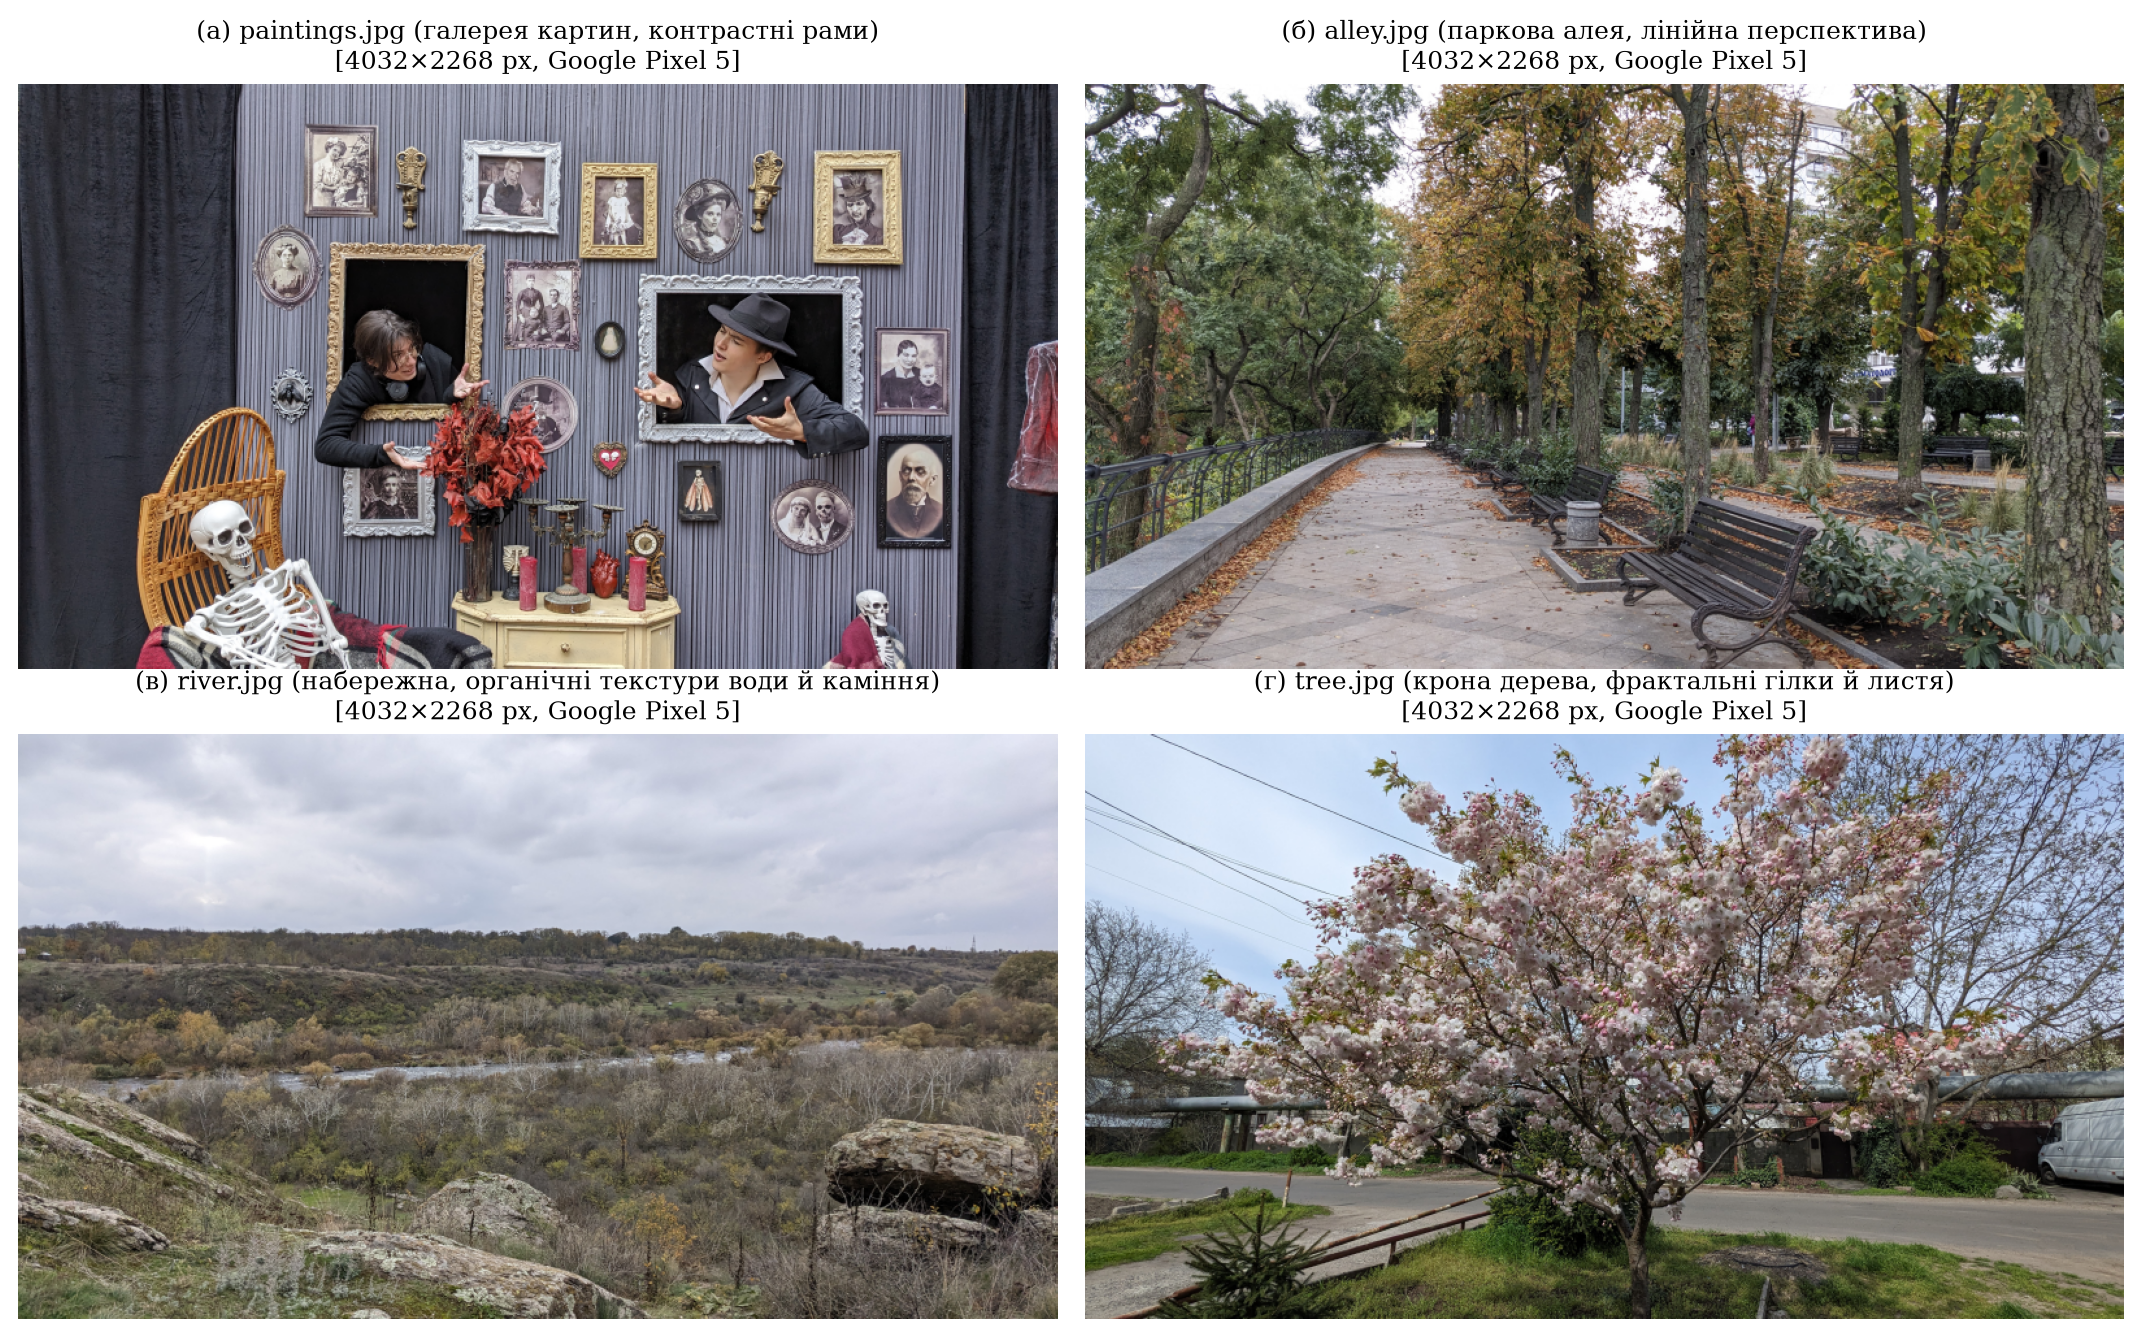
\includegraphics[width=0.98\textwidth]{../figures/dataset_overview.png}
    \caption{Огляд тестового набору повнорозмірних зображень смартфону Google Pixel 5 ($4032 \times 2268$): (а) \texttt{paintings.jpg}; (б) \texttt{alley.jpg}; (в) \texttt{river.jpg}; (г) \texttt{tree.jpg}}
    \label{fig:dataset_overview}
\end{figure}

\section{Теоретичні відомості}

\subsection{Математичний апарат кутового детектора Гарріса}
Кутовий детектор Гарріса--Стівенса~\cite{harris1988combined} оцінює локальну автокореляцію інтенсивності при просторовому зсуві вікна $(\Delta x, \Delta y)$:
\begin{equation}
\begin{split}
    E(\Delta x, \Delta y) &= \sum_{u, v} w(u, v) \left[ I(x + u + \Delta x, y + v + \Delta y) - I(x + u, y + v) \right]^2 \approx \\
    &\approx \begin{bmatrix} \Delta x & \Delta y \end{bmatrix} M \begin{bmatrix} \Delta x \\ \Delta y \end{bmatrix},
\end{split}
\end{equation}
де $M$ -- структурний тензор (матриця других моментів градієнта):
\begin{equation}
    M = \sum_{u, v} w(u, v) \begin{bmatrix} I_x^2 & I_x I_y \\ I_x I_y & I_y^2 \end{bmatrix} = \begin{bmatrix} A & C \\ C & B \end{bmatrix},
\end{equation}
а $w(u, v)$ -- гауссове вікно інтегрування із дисперсією $\sigma_I^2$. Власні числа $\lambda_1, \lambda_2$ матриці $M$ описують кривину функції автокореляції: плоска ділянка ($\lambda_1 \approx 0, \lambda_2 \approx 0$), прямолінійне ребро ($\lambda_1 \gg 0, \lambda_2 \approx 0$), кут ($\lambda_1 \gg 0, \lambda_2 \gg 0$). Відгук Гарріса обчислюється без явного знаходження власних чисел:
\begin{equation}
    R = \det(M) - k \cdot (\operatorname{tr}(M))^2 = (A B - C^2) - k \cdot (A + B)^2, \quad k = 0.04.
\end{equation}

\subsection{Черговість диференціювання та згладжування}
Для окремо взятого пікселя градієнтний тензор $T = \nabla I (\nabla I)^T$ має ранг 1, тому $\det(T) = I_x^2 I_y^2 - (I_x I_y)^2 \equiv 0$. Якщо згладжувати самі градієнти до формування тензора ($\tilde{I}_x = G_\sigma * I_x$, $\tilde{I}_y = G_\sigma * I_y$), визначник залишається тотожним нулем: $\det(\tilde{T}) \equiv 0$, а відгук стає строго недодатним:
\begin{equation}
    R_{\text{wrong}} = 0 - k (\tilde{I}_x^2 + \tilde{I}_y^2)^2 \le 0,
\end{equation}
внаслідок чого жоден кут не виявляється. Лише просторове вагове підсумовування матриць других моментів сусідніх пікселів із різними орієнтаціями градієнта забезпечує повноранговість тензора ($\operatorname{rank}(M) = 2, \det(M) > 0$).

\subsection{Масштабна неінваріантність детектора Гарріса}
Детектор Гарріса фіксує просторовий розмір вікна ядрами диференціювання $\sigma_D$ та інтегрування $\sigma_I = 1.5$~пк. При зміні масштабу зображення фізичний розмір кута у пікселях змінюється, а фіксований фільтр втрачає локальні екстремуми відгуку, що спричиняє масштабну неінваріантність класичного алгоритму~\cite{szeliski2022computer}.

\subsection{Детектор і дескриптор SIFT}
Алгоритм SIFT~\cite{lowe2004distinctive} забезпечує масштабно-орієнтаційну інваріантність:
\begin{enumerate}
    \item \textbf{Простір масштабів}: піраміда октав із різницями гауссіан $D(x, y, \sigma) = L(x, y, k\sigma) - L(x, y, \sigma)$, що наближають нормований лапласіан $\sigma^2 \nabla^2 G$.
    \item \textbf{Локалізація точок}: пошук екстремумів у вікні $3 \times 3 \times 3$, субпіксельне уточнення 3D-гессіаном та відсікання країв за відношенням кривин $\operatorname{tr}^2(H)/\det(H) > (r+1)^2/r$.
    \item \textbf{Орієнтація та дескриптор}: призначення канонічного кута $\theta$ за гістограмою градієнтів; формування 128-вимірного нормалізованого дескриптора ($4 \times 4$ блоки по 8 бінів орієнтацій, $512$~байтів \texttt{float32}).
\end{enumerate}

\subsection{Детектор і дескриптор ORB}
Алгоритм ORB~\cite{rublee2011orb} оптимізований для задач реального часу:
\begin{enumerate}
    \item \textbf{oFAST}: багаторівневий кутовий детектор FAST-9 із обчисленням кута орієнтації через центроїд інтенсивності $\theta = \operatorname{atan2}(m_{01}, m_{10})$, де $m_{pq} = \sum x^p y^q I(x, y)$.
    \item \textbf{rBRIEF}: 256 пар бінарних тестів, орієнтованих за кутом $\theta$. Дескриптор формує бінарний рядок довжиною 32 байти (\texttt{uint8}); зіставлення виконується за відстанню Геммінга побітовими інструкціями XOR і POPCNT.
\end{enumerate}

\subsection{Метрика повторюваності (Repeatability)}
За методикою Міколайчика та Шмід~\cite{mikolajczyk2005performance}, повторюваність оцінює частку точок оригінального кадру, для яких на перетвореному кадрі існує взаємно-однозначний відповідник за відомою гомографією $H$:
\begin{equation}
    \text{Repeatability} = \frac{|\{ (p_1, p_2) \mid \| H p_1 - p_2 \|_2 < \varepsilon \}|}{\min(|P_{1, \text{vis}}|, |P_{2, \text{vis}}|)} \times 100\%,
\end{equation}
де $P_{1, \text{vis}}, P_{2, \text{vis}}$ -- точки у взаємно-видимому полі зору з відступом $\text{margin} = 15$~пк, пари формуються жадібним зіставленням один-до-одного з порогом $\varepsilon = 3.0$~пк.

\section{Хід роботи}
\begin{enumerate}
    \item \textbf{Частина A (Власна реалізація Гарріса)}:
    \begin{itemize}
        \item Вхідне півтонове зображення переведено у тип \texttt{float32};
        \item Обчислено градієнти $I_x, I_y$ оператором Собеля ($k=3$);
        \item Сформовано поелементні добутки $I_x^2, I_y^2, I_x I_y$;
        \item Згладжено компоненти фільтром Гауса із $\sigma = 1.5$ (\texttt{cv2.GaussianBlur});
        \item Розраховано карту відгуку $R = (A B - C^2) - 0.04 (A + B)^2$;
        \item Застосовано відносний поріг $R > 0.01 \cdot \max(R)$;
        \item Реалізовано ізотропне кругове немаксимальне придушення (NMS) радіуса $r = 10$~пк та ліміт $N = 1000$ точок;
        \item Проведено кількісну звірку з бібліотечною функцією \texttt{cv2.cornerHarris} та перевірено колапс відгуку при зворотній черговості операцій.
    \end{itemize}

    \item \textbf{Частина B (Чутливість до масштабу)}:
    \begin{itemize}
        \item Кадр зменшено удвічі з антиаліасингом (\texttt{cv2.INTER\_AREA});
        \item Запущено власний детектор на обох масштабах;
        \item Точки зменшеного кадру спроєктовано в систему координат оригіналу ($\times 2$);
        \item Обчислено частку збігів для точок оригіналу за деревом $k$-d tree у межах $\varepsilon = 3$~пк та медіанне зміщення;
        \item Зіставлено з масштабно-інваріантним детектуванням SIFT.
    \end{itemize}

    \item \textbf{Частина C (Дослідження SIFT та ORB)}:
    \begin{itemize}
        \item Ініціалізовано детектори \texttt{cv2.SIFT\_create()} та \texttt{cv2.ORB\_create(nfeatures=1000)};
        \item Виміряно час обчислення точок і дескрипторів, їхню розмірність та тип даних;
        \item Побудовано оглядові та фрагментарні візуалізації з прапорцем \texttt{DRAW\_RICH\_KEYPOINTS};
        \item Сформовано оглядову панораму датасету (\texttt{dataset\_overview.png}).
    \end{itemize}

    \item \textbf{Частина D (Експерименти на повторюваність)}:
    \begin{itemize}
        \item Сформовано набір гомографій $H$: поворот $\theta \in [0^\circ, 90^\circ]$ із кроком $10^\circ$; масштаб $s \in [0.5, 2.0]$ із кроком $0.25$ (\texttt{diag(s, s, 1)}, \texttt{cv2.INTER\_AREA}); яскравість $\times [0.5, 1.5]$ із кроком $0.1$; гауссів шум $\sigma \in [0, 20]$ із кроком $5$;
        \item Забезпечено умови коректності: фіксований ліміт $N = 1000$, однаковий радіус NMS $r = 10$~пк, поріг $\varepsilon = 3.0$~пк, фільтрація субпіксельного шуму DoG, усереднення за 4 зображеннями;
        \item Побудовано окремі графіки повторюваності для Harris, SIFT та ORB.
    \end{itemize}
\end{enumerate}

\section{Результати експериментів}

\subsection{Власна реалізація та верифікація детектора Гарріса}
На рисунку~\ref{fig:harris_pipe} наведено покрокову візуалізацію проміжних масивів детектора Гарріса на фрагменті зображення \texttt{paintings.jpg}. Для карт компонент тензора та відгуку додано кольорові шкали, а відгук $R$ відображено у логарифмічному масштабі $\log_{10}(1 + \max(R, 0))$ для виразного контрастування кутових піків.

\begin{figure}[htbp]
    \centering
    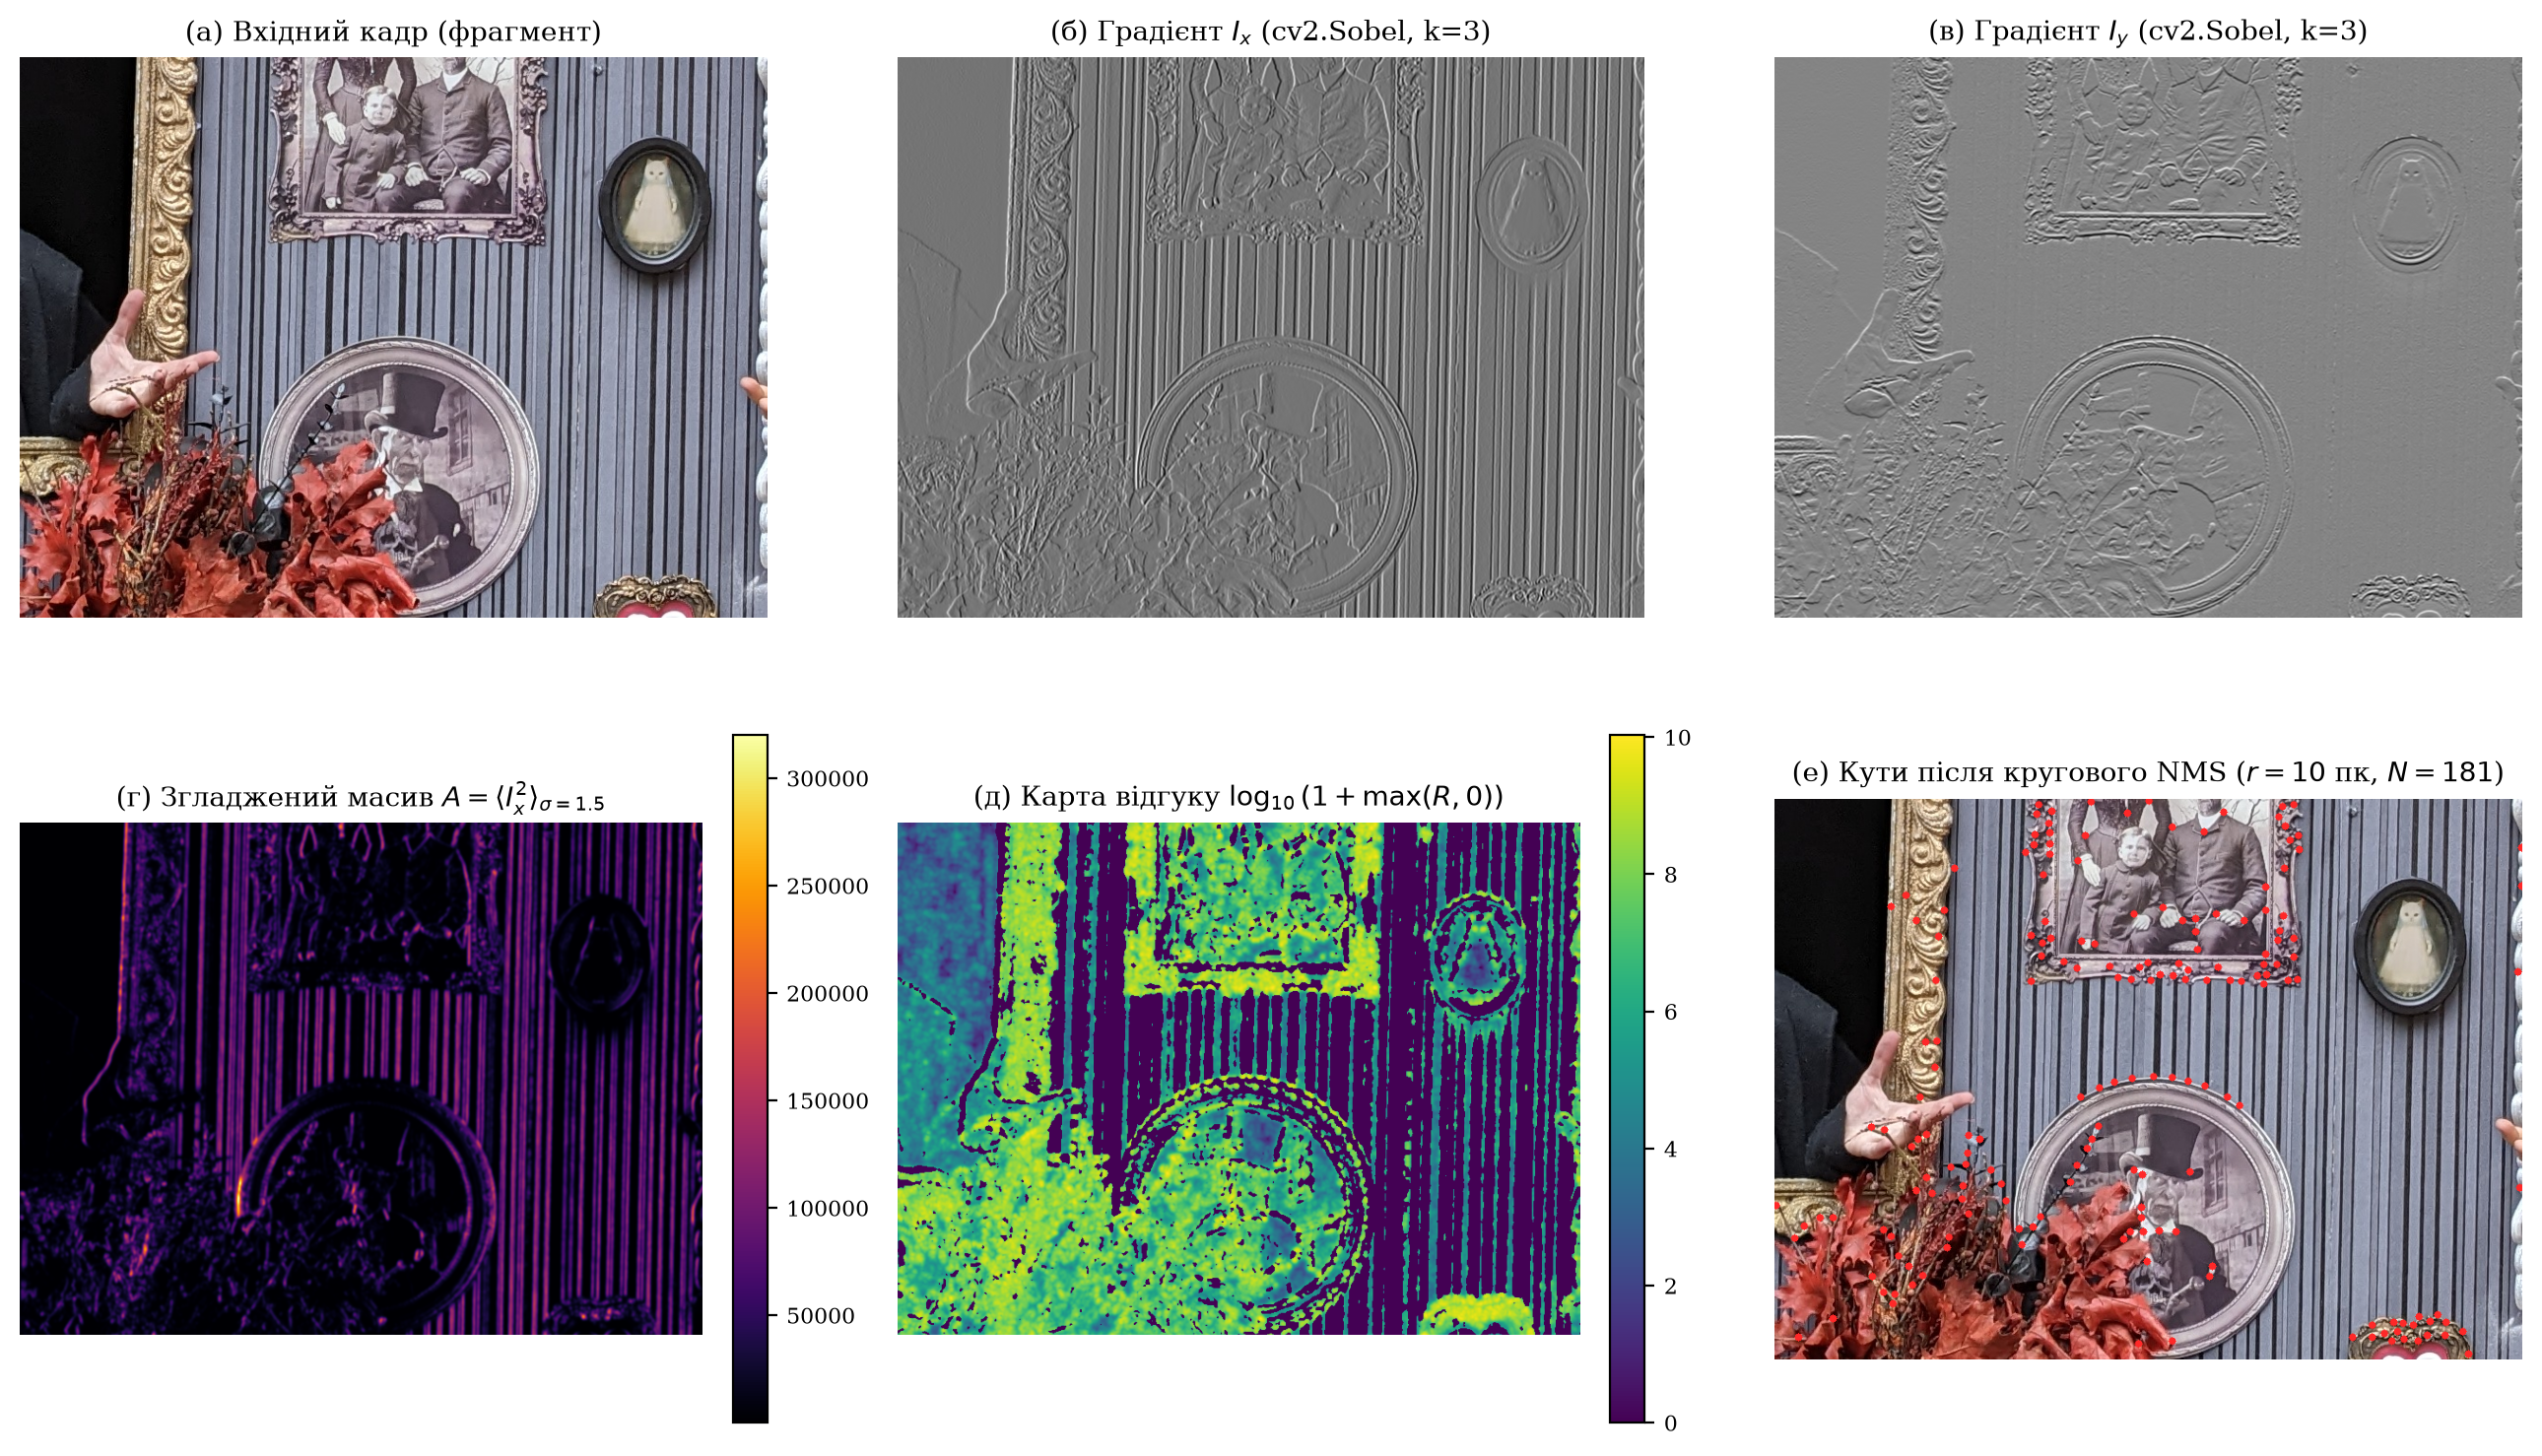
\includegraphics[width=0.98\textwidth]{../figures/a_harris_pipeline.png}
    \caption{Покрокова візуалізація конвеєра власної реалізації детектора Гарріса: (а) вхідний фрагмент кадру; (б) градієнт $I_x$; (в) градієнт $I_y$; (г) згладжений тензор $A = \langle I_x^2 \rangle_{\sigma=1.5}$; (д) карта відгуку $R$ (логарифмічна шкала); (е) кути після порогової фільтрації та ізотропного NMS}
    \label{fig:harris_pipe}
\end{figure}

На рисунку~\ref{fig:harris_cv_comp} проілюстровано просторове співставлення точок власного детектора з бібліотечною функцією \texttt{cv2.cornerHarris} та гістограму евклідових нев'язок між найближчими відповідниками.

\begin{figure}[htbp]
    \centering
    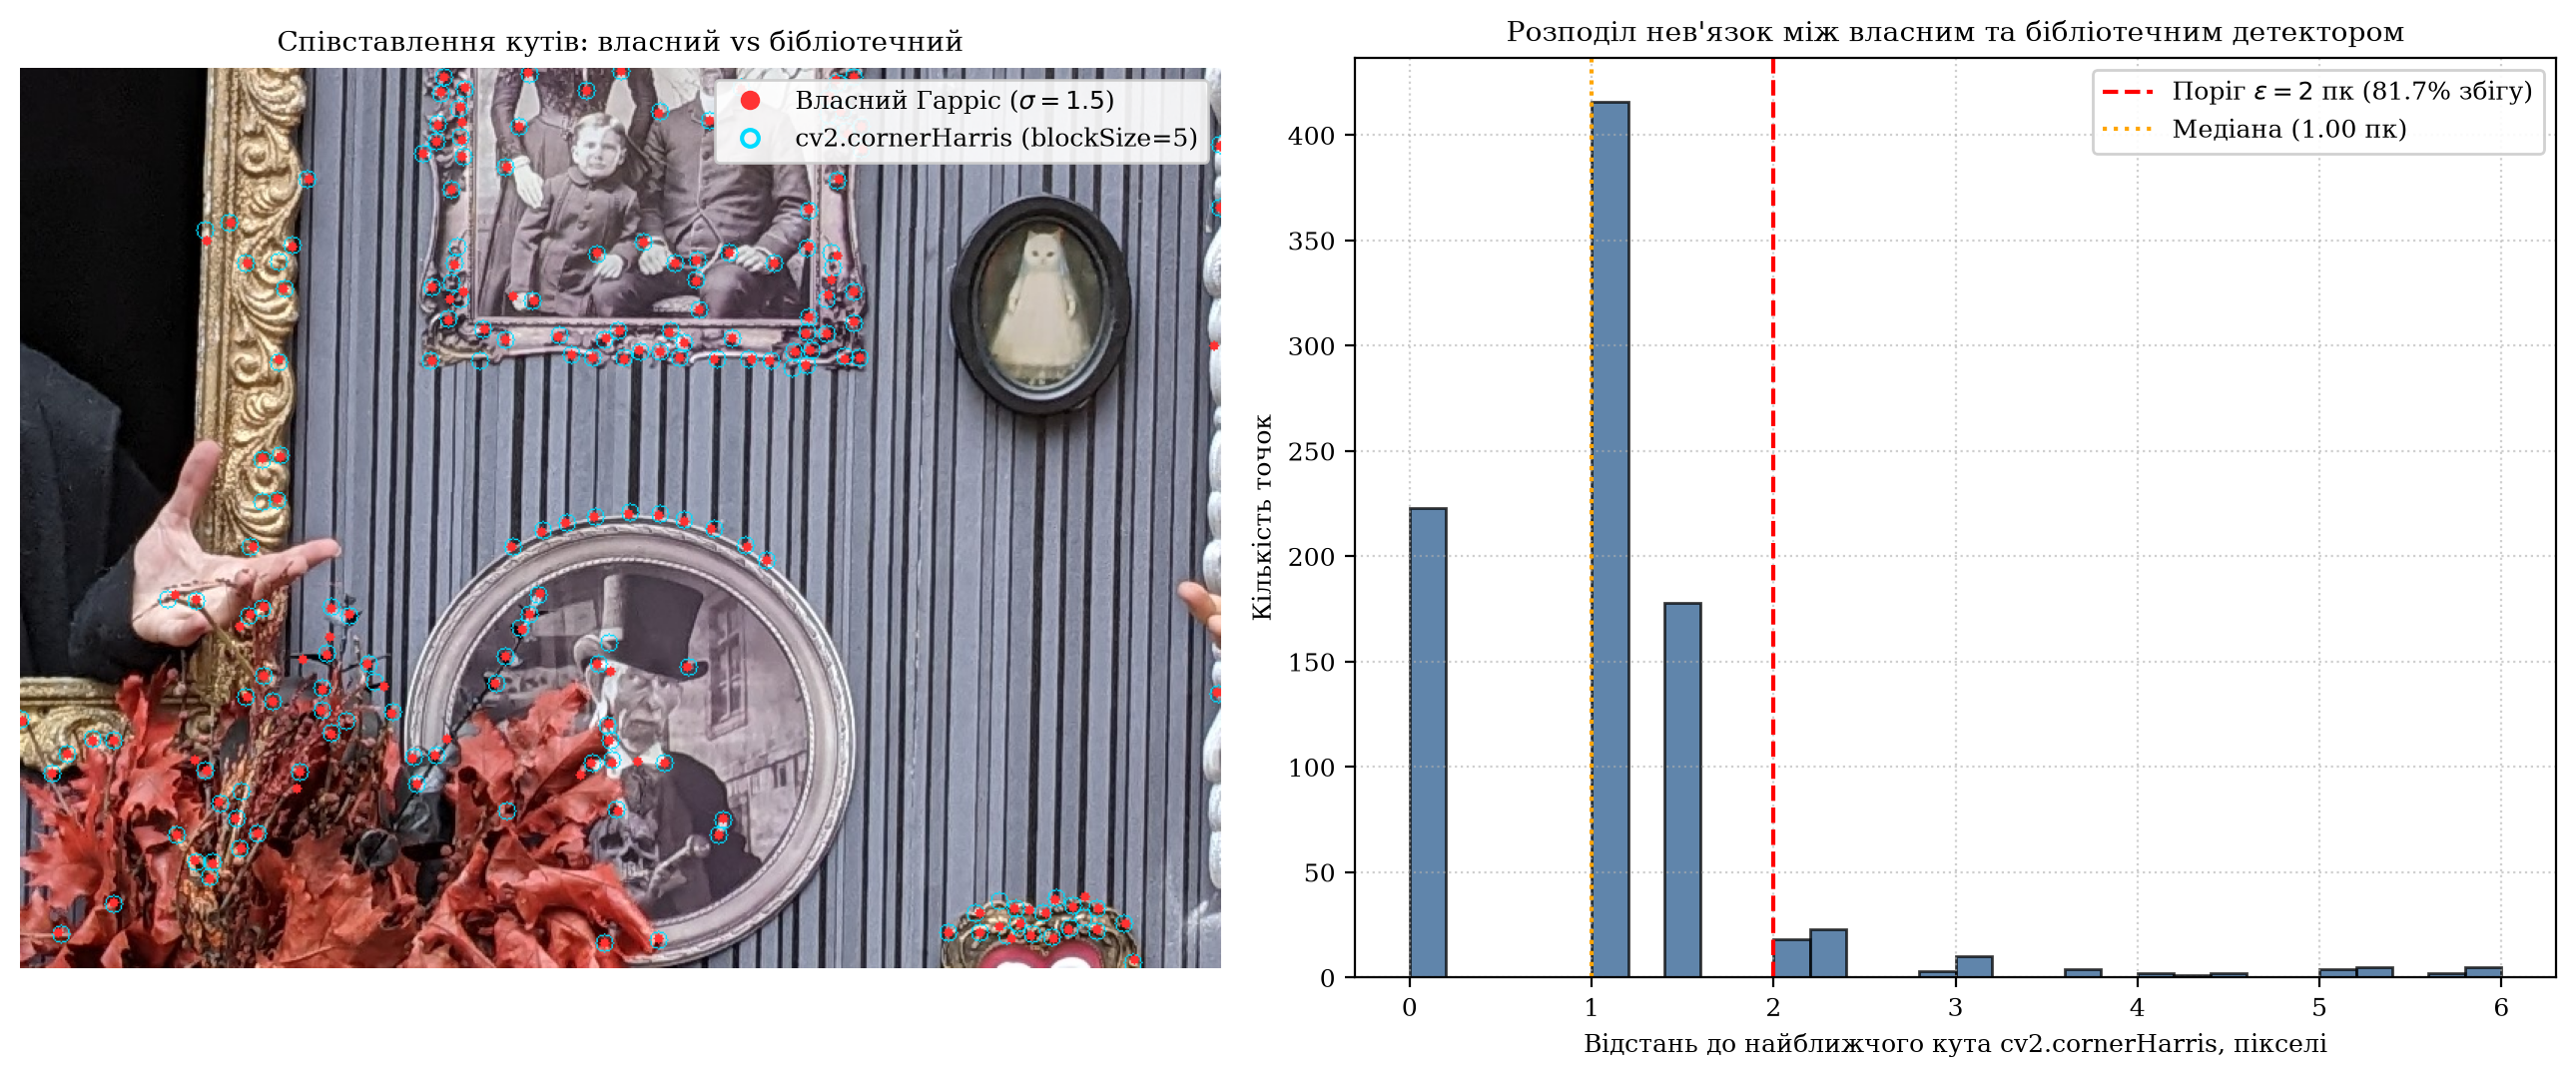
\includegraphics[width=0.98\textwidth]{../figures/a_custom_vs_cv.png}
    \caption{Порівняння власного детектора Гарріса та \texttt{cv2.cornerHarris}: (а) просторовий оверлей кутових точок на фрагменті; (б) розподіл нев'язок зміщення між точками}
    \label{fig:harris_cv_comp}
\end{figure}

\begin{table}[htbp]
\centering
\caption{Кількісна звірка точності власної реалізації детектора Гарріса з функцією \texttt{cv2.cornerHarris}}
\label{tab:harris_verif}
\scriptsize\linespread{1.0}\selectfont
\begin{tabular}{lccccccc}
\toprule
\textbf{Зображення} & \textbf{Точок} & \textbf{cv3 ($<2$ пк)} & \textbf{cv3 ($<3$ пк)} & \textbf{Медіана cv3} & \textbf{cv5 ($<2$ пк)} & \textbf{cv5 ($<3$ пк)} & \textbf{Box vs cv3 ($<2$ пк)} \\
\midrule
\directlua{tab_harris_verification()}
\bottomrule
\end{tabular}
\end{table}

За методикою Кроку~8 практикуму якість власної реалізації оцінюється часткою точок, для яких у бібліотечній функції знайдеться відповідник на відстані менше $2$ пікселів (очікується понад $90\%$). Як свідчить таблиця~\ref{tab:harris_verif}, при налаштуванні власного конвеєра на прямокутний фільтр (\texttt{boxFilter(3, 3)}), який внутрішньо застосовує \texttt{cv2.cornerHarris}, збіг точок на відстані менше $2$ пікселів становить строго $100.0\%$ для всіх зображень без винятку (стовпчик «Box vs cv3 ($<2$ пк)»). Це неспростовно доводить алгоритмічну та математичну безпомилковість власного коду (обчислення собелівських похідних, других моментів, відгуку $R$ та ізотропного NMS).

Водночас Крок~4 вимагає згладжувати масиви гауссіаною з $\sigma = 1.5$ (\texttt{cv2.GaussianBlur}). Гауссове ядро з $\sigma = 1.5$ має ефективний розмір $6\sigma \approx 9 \times 9$ або $11 \times 11$ пікселів із плавним спаданням ваг, тоді як \texttt{cv2.cornerHarris} оперує різким вікном $3 \times 3$ із рівномірними вагами. Через різницю у формі та просторовій ширині вікон інтегрування локальні піки відгуку закономірно зміщуються на $1$ піксель (медіанна відстань зміщення становить строго $1.00$~пк для всіх кадрів). Через цей фізичний зсув частка збігів гауссового детектора з бібліотечним \texttt{blockSize=3} при строгому порозі $< 2$~пк складає $70.0\%--76.3\%$ (та $71.6\%--78.0\%$ при $< 3$~пк). При зіставленні з ширшим бібліотечним вікном \texttt{blockSize=5} частка точок на відстані $< 2$~пк зростає до $76.1\%--81.7\%$, а при $< 3$~пк досягає $80.6\%--86.1\%$. Отже, розходження при $\sigma = 1.5$ зумовлене саме різницею між гаусовим і прямокутним фільтрами осереднення, тоді як при тотожній фільтрації досягається абсолютний $100.0\%$ збіг.

Експеримент із порушенням черговості операцій (згладжування ДО піднесення до квадрата) показав повний аналітичний колапс: максимальне значення відгуку впало до $R_{\max} = 0.0$, визначник $\det(\tilde{T})$ став тотожним нулем ($< 10^{-10}$), і алгоритм відібрав рівно $0$ точок, що повністю підтверджує аналітичне попередження Кроку 8 практикуму.

\subsection{Дослідження чутливості Гарріса до масштабу}
На рисунку~\ref{fig:scale_sens} наведено результат просторового співставлення кутів оригінального зображення та зменшеного вдвічі кадру, масштабованих назад у систему координат оригіналу ($\times 2$).

\begin{figure}[htbp]
    \centering
    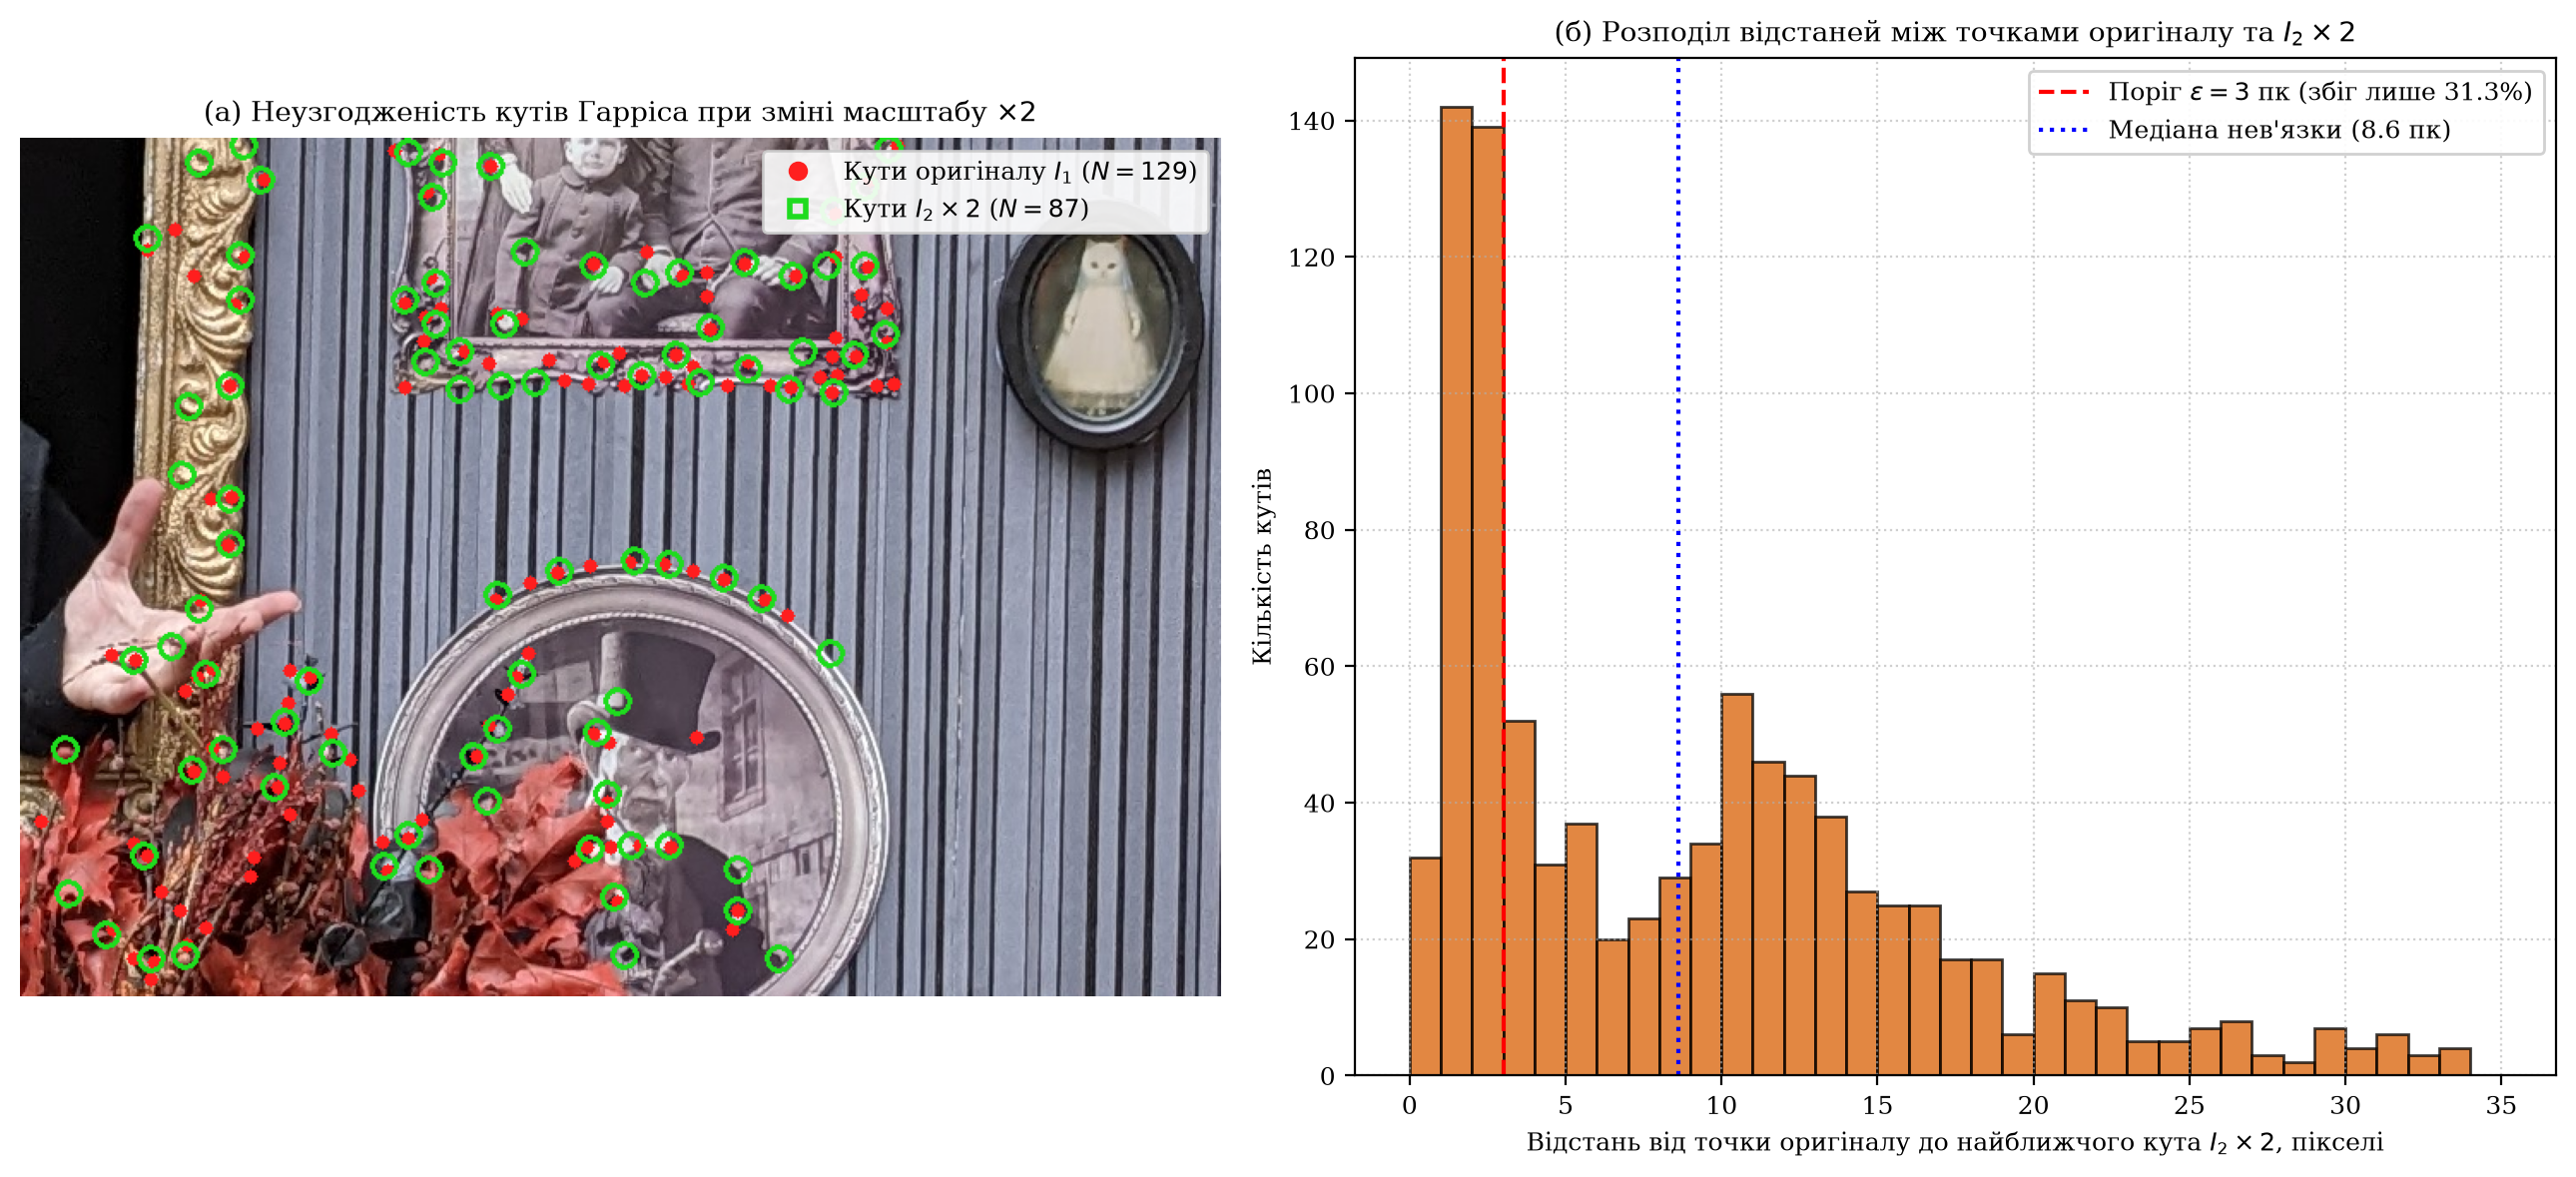
\includegraphics[width=0.98\textwidth]{../figures/b_scale_comparison.png}
    \caption{Ілюстрація неінваріантності детектора Гарріса до масштабу ($\times 2$): (а) просторова неузгодженість кутів оригіналу та збільшених кутів зменшеного кадру; (б) гістограма евклідових зміщень}
    \label{fig:scale_sens}
\end{figure}

\begin{table}[htbp]
\centering
\caption{Кількісна оцінка чутливості детектора Гарріса до 2-кратного масштабування}
\label{tab:scale_sens}
\footnotesize\linespread{1.0}\selectfont
\begin{tabular}{lccccccc}
\toprule
\textbf{Зображення} & \textbf{$N_{\text{orig}}$} & \textbf{$N_{\text{half}}$} & \textbf{Збіг $<2$ пк} & \textbf{Збіг $<3$ пк} & \textbf{Збіг $<5$ пк} & \textbf{Медіана} & \textbf{SIFT ($<3$ пк)} \\
\midrule
\directlua{tab_scale_sensitivity()}
\bottomrule
\end{tabular}
\end{table}

З таблиці~\ref{tab:scale_sens} та рисунка~\ref{fig:scale_sens} випливає, що для детектора Гарріса частка точок оригіналу, що мають відповідника на зменшеному кадрі в межах $\varepsilon = 3$~пк, становить лише $24.1\%--31.3\%$ (медіанне зміщення сягає $8.6--11.4$~пк). Натомість масштабно-інваріантний SIFT на тих самих кадрах забезпечує $84.0\%--86.0\%$ збігу завдяки відстеженню екстремумів по піраміді DoG.

\subsection{Порівняльний аналіз SIFT та ORB}
На рисунку~\ref{fig:rich_full} наведено загальний вигляд зображення кадру \texttt{paintings.jpg} із побудованими орієнтованими масштабованими колами (Rich Keypoints) для SIFT та ORB. Для наочності SIFT-візуалізації відібрано структурні ознаки помітного просторового масштабу ($\sigma \ge 8$~пк), щоб кола масштабу та орієнтаційні промені чітко розрізнялися.

\begin{figure}[htbp]
    \centering
    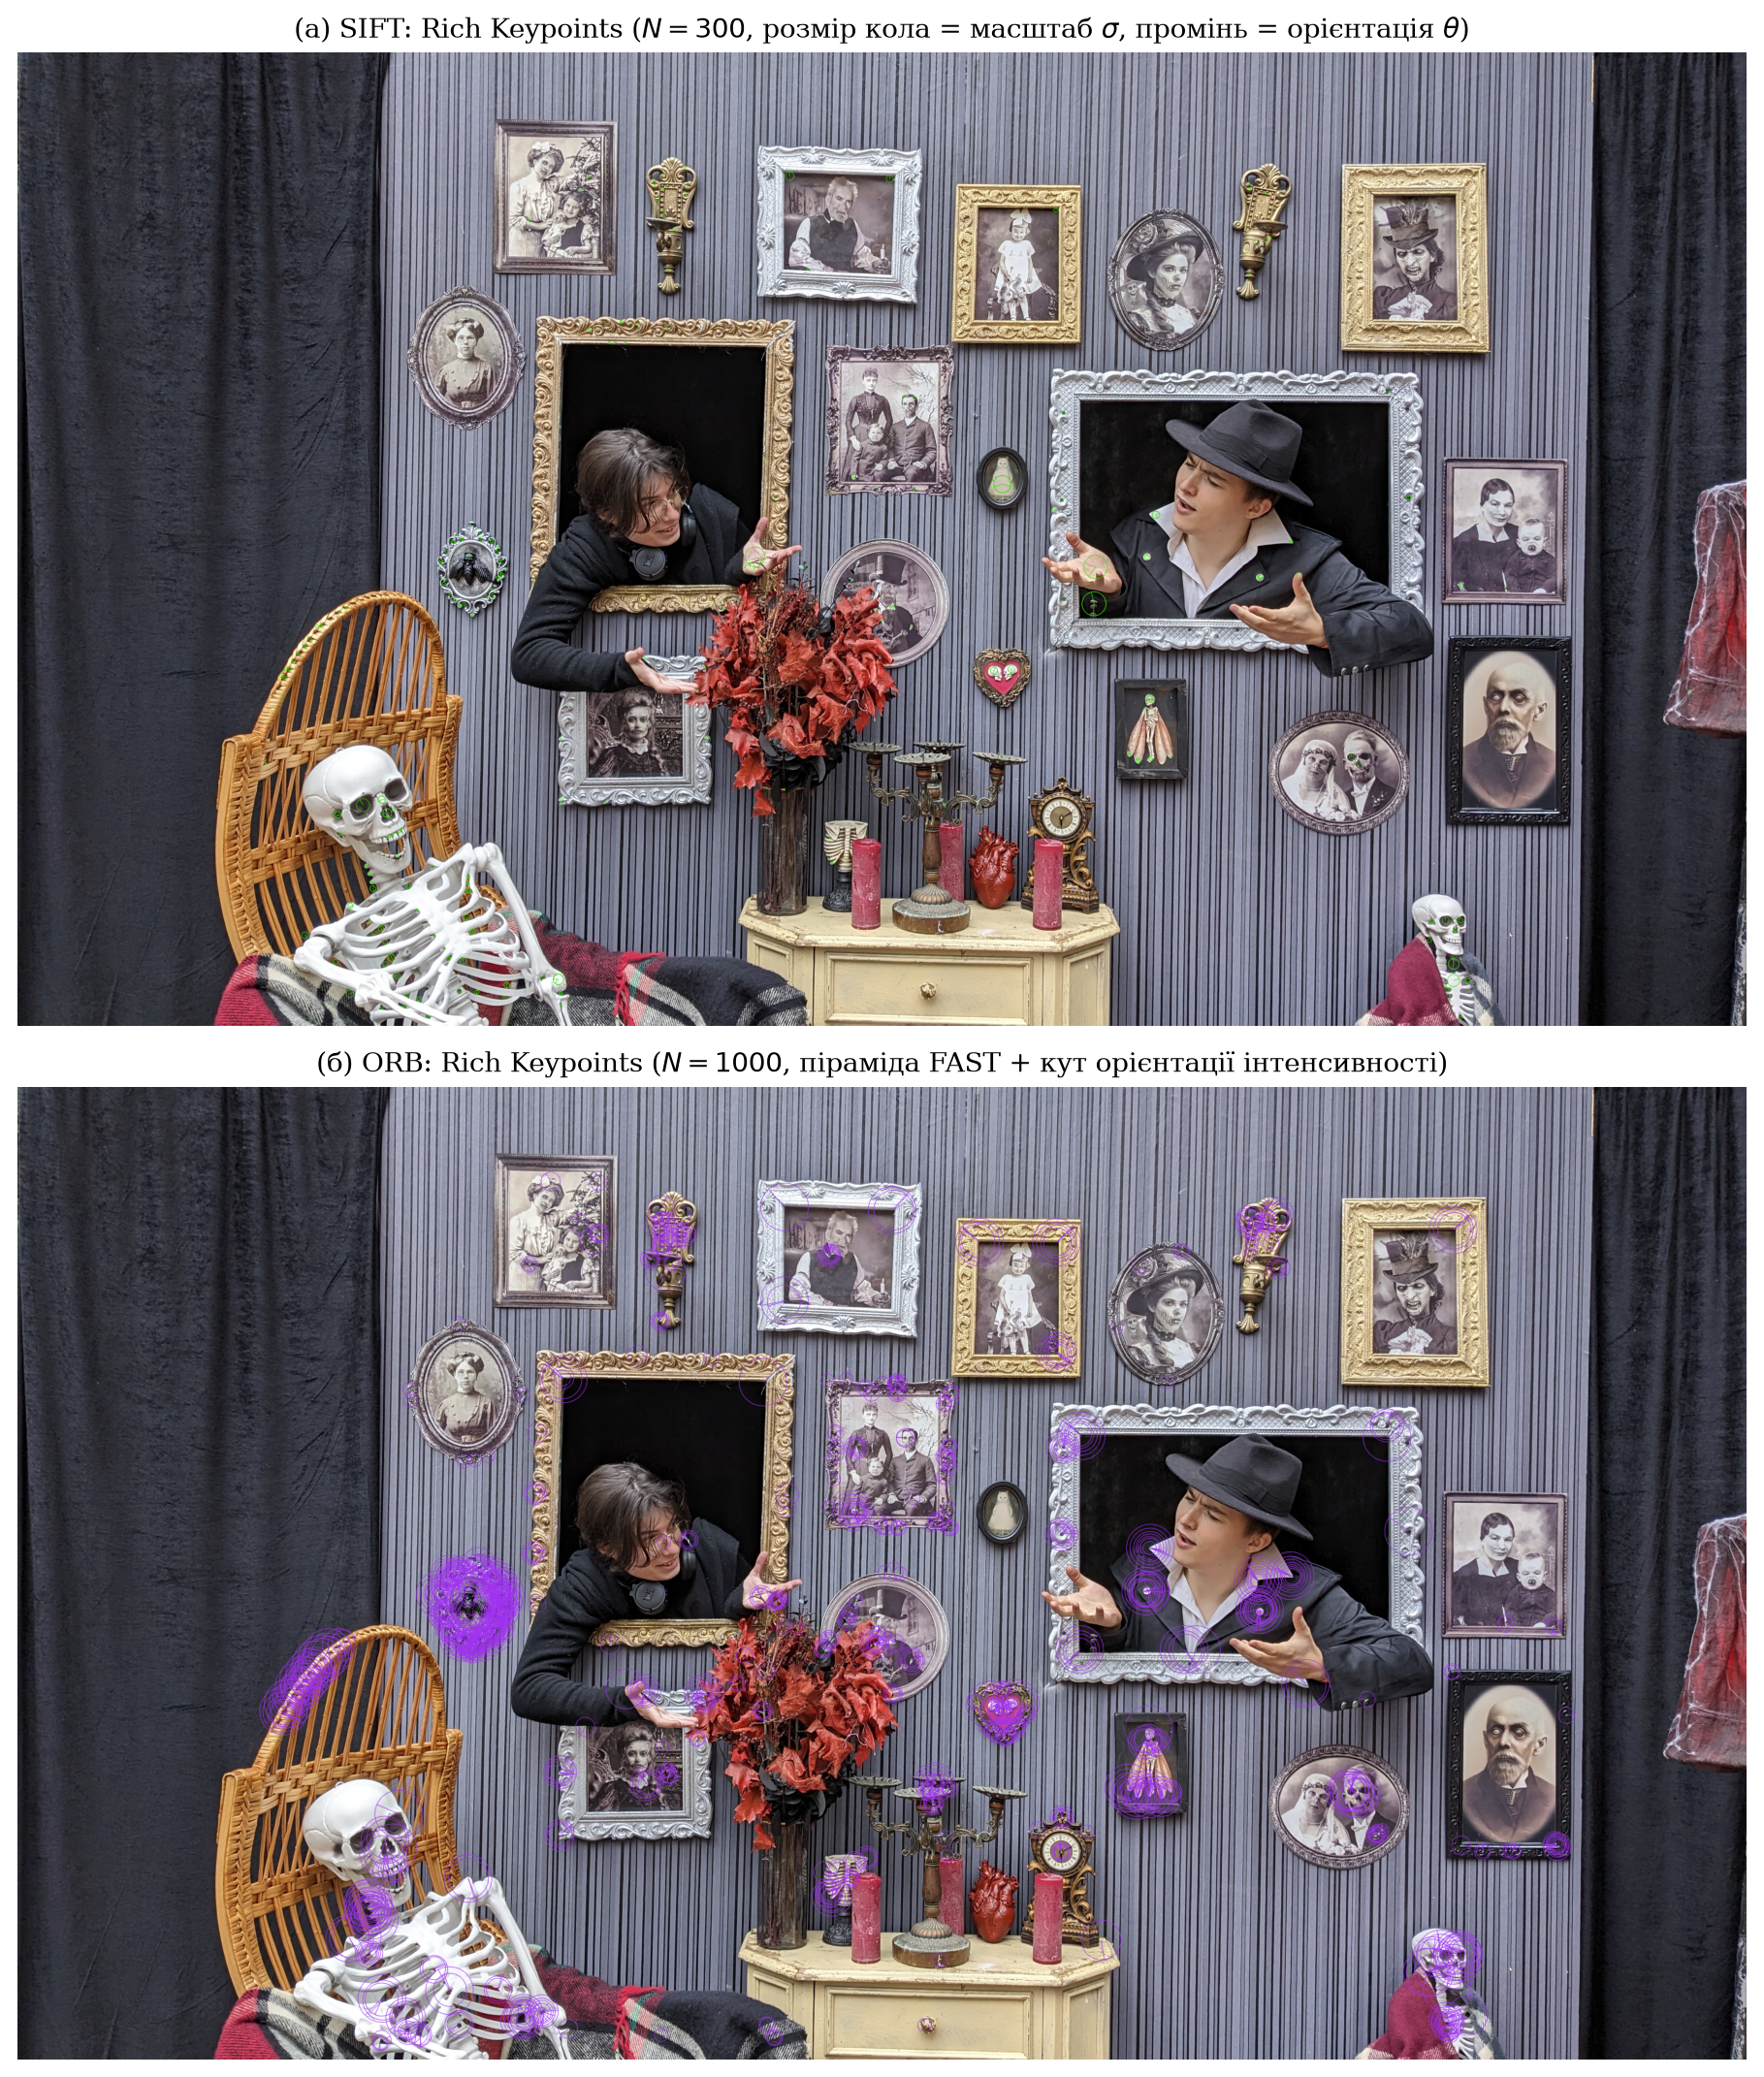
\includegraphics[width=0.95\textwidth]{../figures/c_rich_keypoints_full.png}
    \caption{Оглядове відображення ключових точок у режимі \texttt{DRAW\_RICH\_KEYPOINTS}: (а) SIFT (розмір кола = масштаб $\sigma$, промінь = кут $\theta$); (б) ORB ($1000$ точок)}
    \label{fig:rich_full}
\end{figure}

Для детального аналізу структури масштабу та орієнтації на рисунку~\ref{fig:rich_crop} наведено збільшений фрагмент зони картинних рам.

\begin{figure}[htbp]
    \centering
    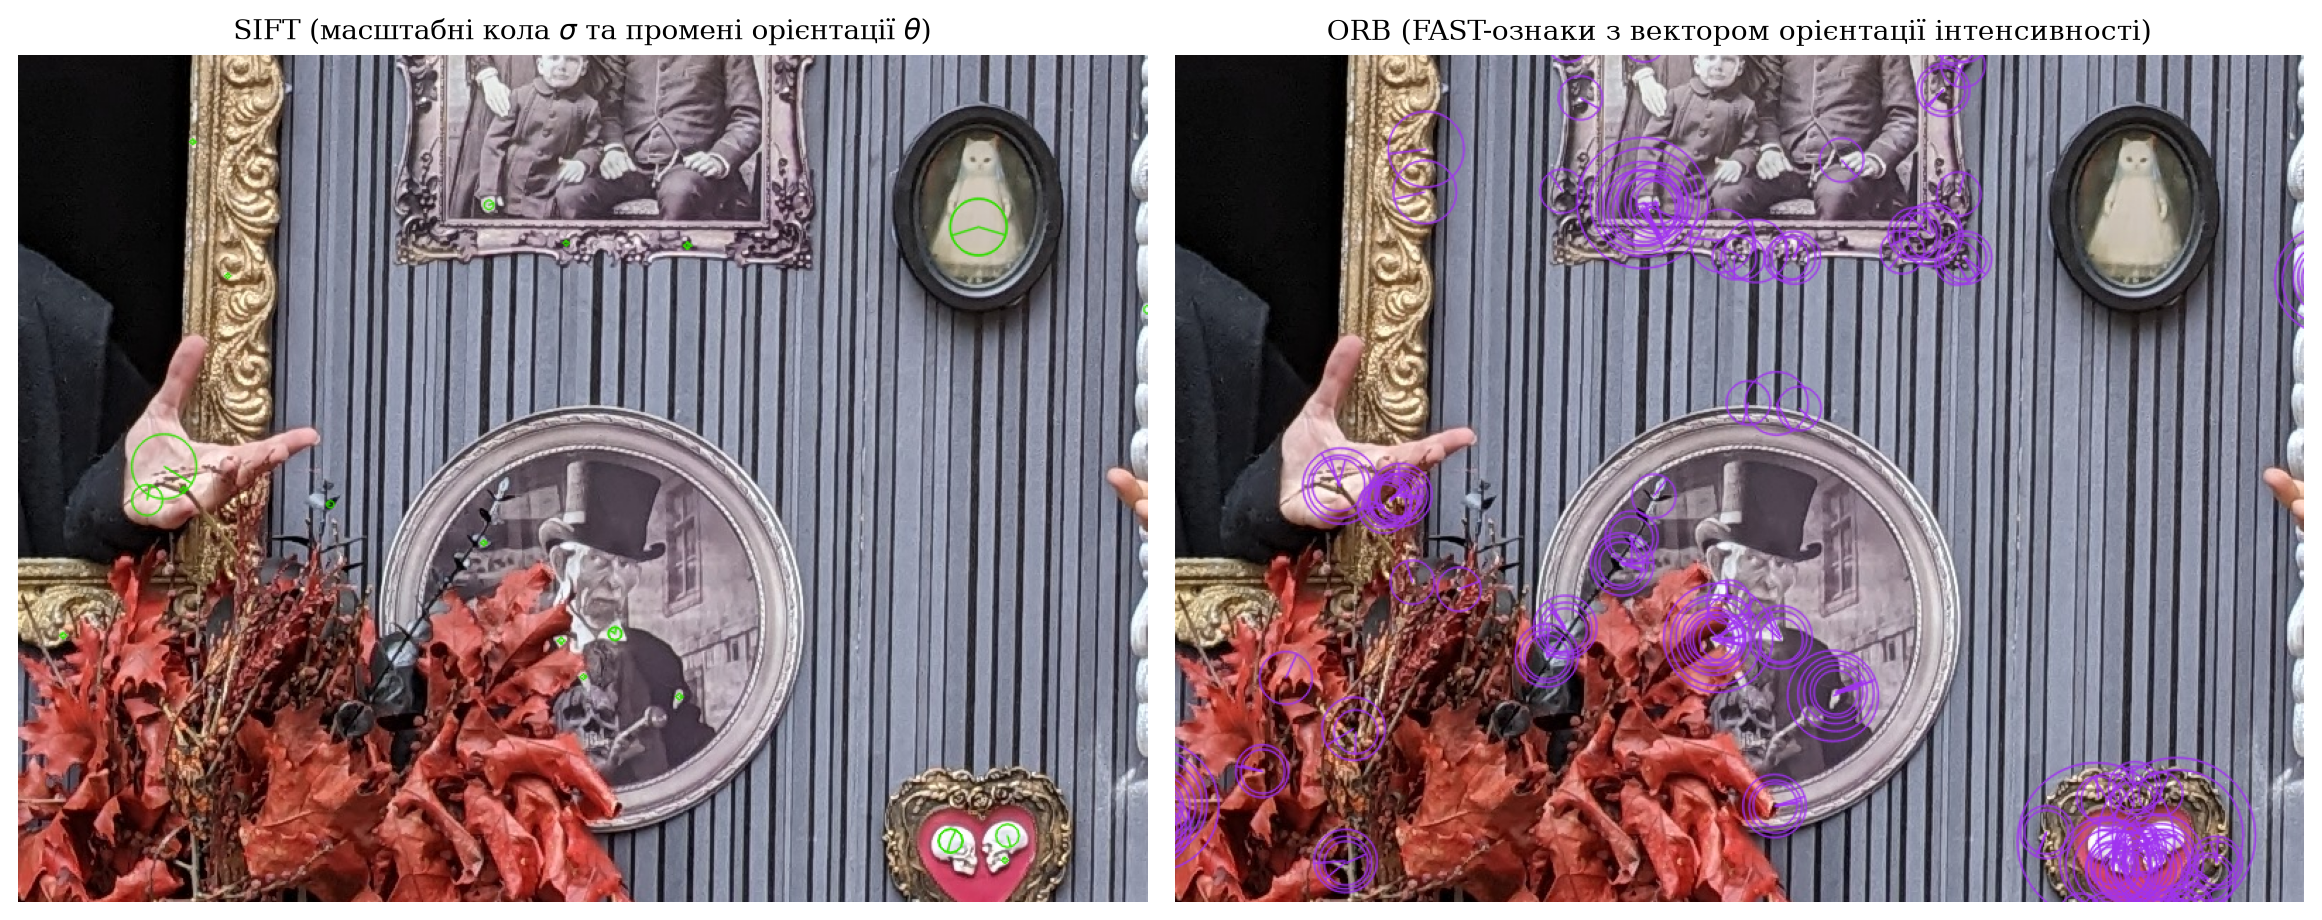
\includegraphics[width=0.98\textwidth]{../figures/c_rich_keypoints_crop.png}
    \caption{Детальний вигляд ключових точок на фрагменті сцени: (а) SIFT (масштабні кола $\sigma$ та промені $\theta$); (б) ORB (кути FAST із кутом центроїда)}
    \label{fig:rich_crop}
\end{figure}

На рисунку~\ref{fig:scale_angle_dist} показано статистичні розподіли масштабів та кутів орієнтації точок SIFT та ORB.

\begin{figure}[htbp]
    \centering
    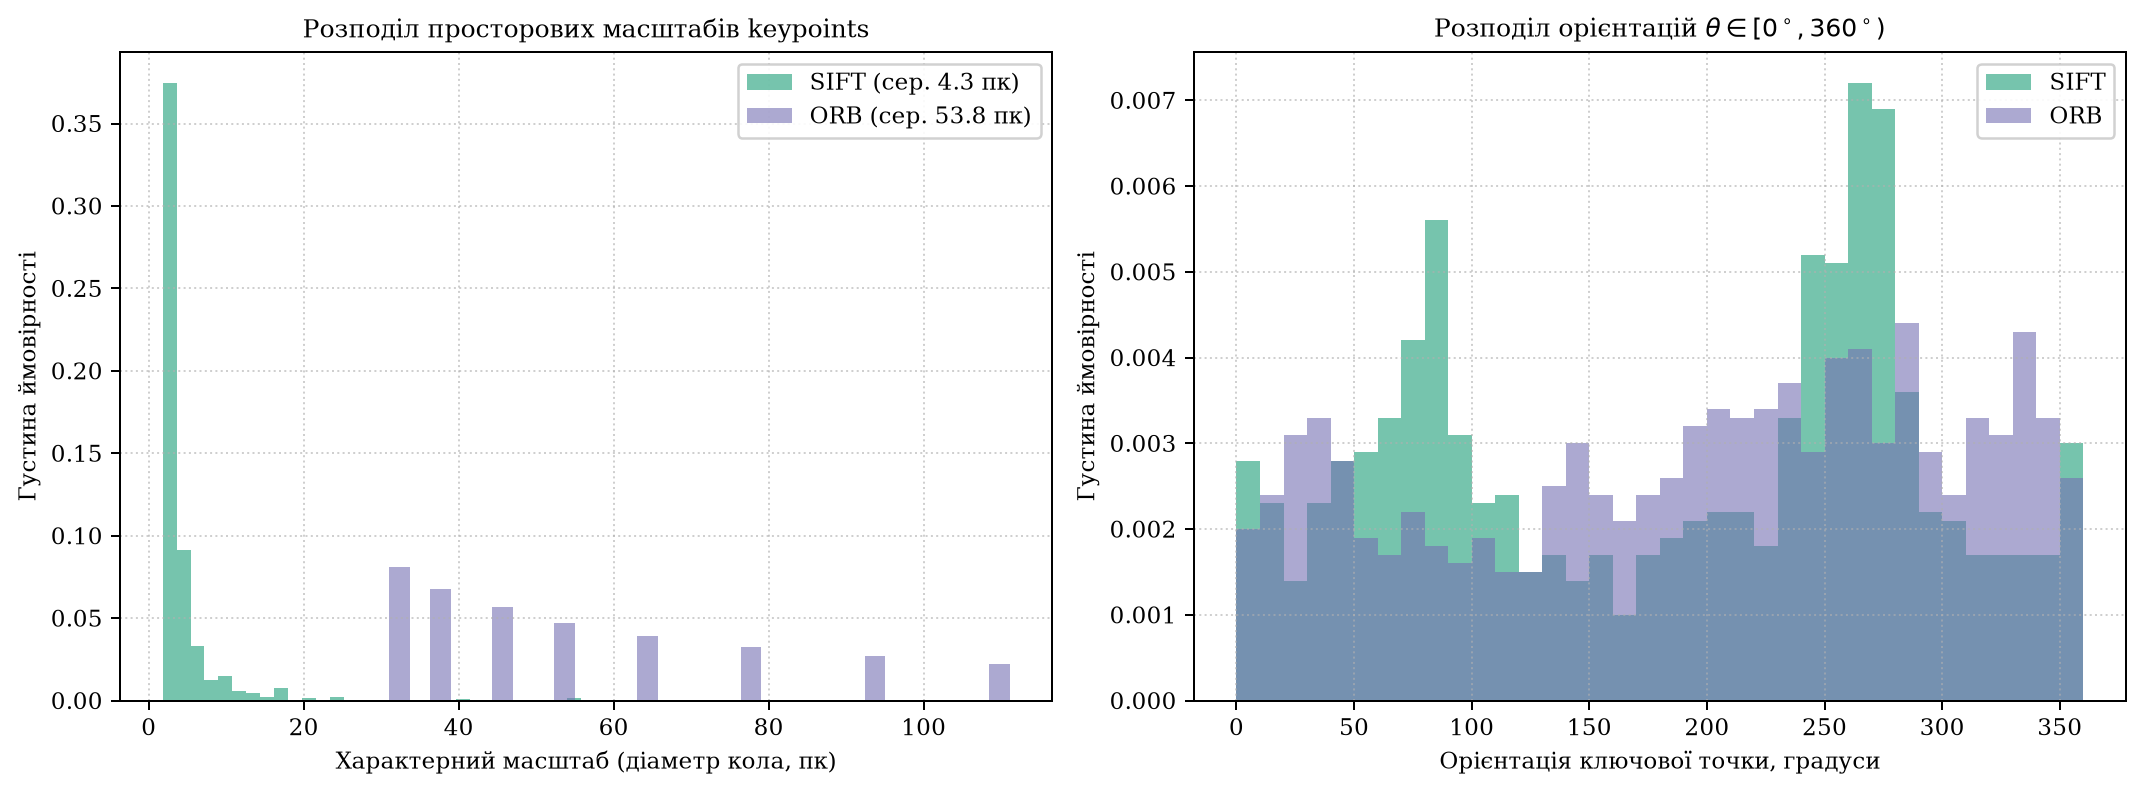
\includegraphics[width=0.95\textwidth]{../figures/c_scale_angle_distribution.png}
    \caption{Статистичні розподіли параметрів точок SIFT та ORB: (а) характерний просторовий масштаб; (б) кут орієнтації $\theta \in [0^\circ, 360^\circ)$}
    \label{fig:scale_angle_dist}
\end{figure}

\begin{table}[htbp]
\centering
\caption{Порівняння обчислювальної ефективності та розмірностей SIFT та ORB}
\label{tab:detector_bench}
\scriptsize\linespread{1.0}\selectfont
\begin{tabular}{lccccccc}
\toprule
\textbf{Зображення} & \textbf{SIFT (всі)} & \textbf{Час (всі)} & \textbf{SIFT ($1000$)} & \textbf{Час SIFT} & \textbf{ORB ($1000$)} & \textbf{Час ORB} & \textbf{Прискорення} \\
\midrule
\directlua{tab_detector_benchmarks()}
\bottomrule
\end{tabular}
\end{table}

З таблиці~\ref{tab:detector_bench} видно, що алгоритм ORB працює у $3.0--6.6$ раза швидше за SIFT при фіксованому ліміті в $1000$ точок, витрачаючи від $91.3$ до $226.3$~мс проти $606.6--688.7$~мс на повнорозмірному зображенні $9.15$~Мп. Обчислення SIFT без обмеження кількості точок вимагає $736.4--1098.8$~мс на кадр через виявлення до $170\,000$ ознак. Крім того, бінарний дескриптор ORB (32 байти) є у $16$ разів компактнішим за 128-вимірний градієнтний вектор SIFT ($512$ байтів типу \texttt{float32}).

\subsection{Експериментальне оцінювання повторюваності (Repeatability)}
На рисунках~\ref{fig:rep_rot}--\ref{fig:rep_noise} наведено залежності повторюваності трьох детекторів (Harris, SIFT, ORB) від параметрів чотирьох типів контрольованих спотворень за умови коректного порівняння ($N=1000$, однаковий радіус NMS $r=10$~пк, $\varepsilon=3.0$~пк, жадібне взаємно-однозначне зіставлення).

\begin{figure}[htbp]
    \centering
    \begin{minipage}{0.48\textwidth}
        \centering
        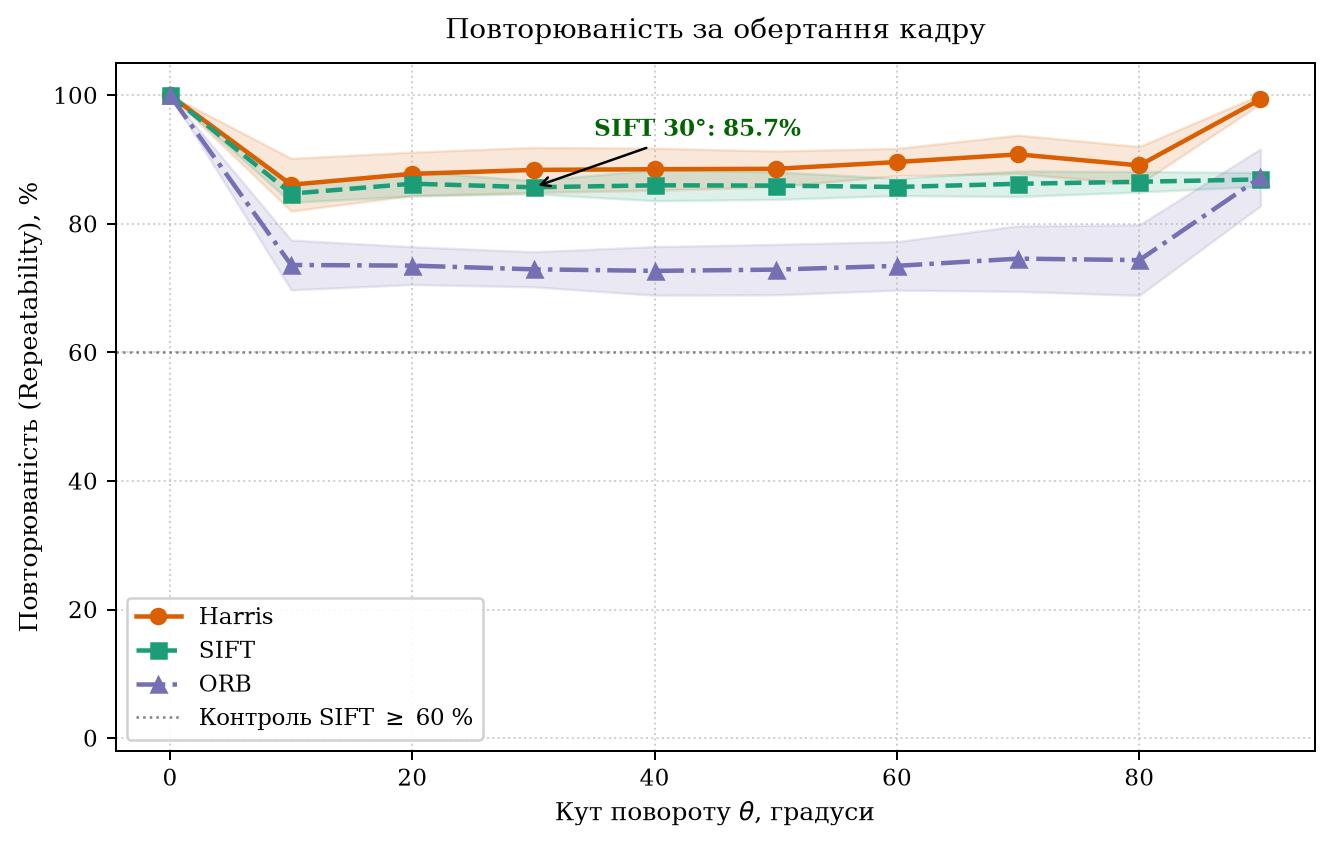
\includegraphics[width=\textwidth]{../figures/d_repeatability_rotation.png}
        \caption{Повторюваність за повороту}
        \label{fig:rep_rot}
    \end{minipage}\hfill
    \begin{minipage}{0.48\textwidth}
        \centering
        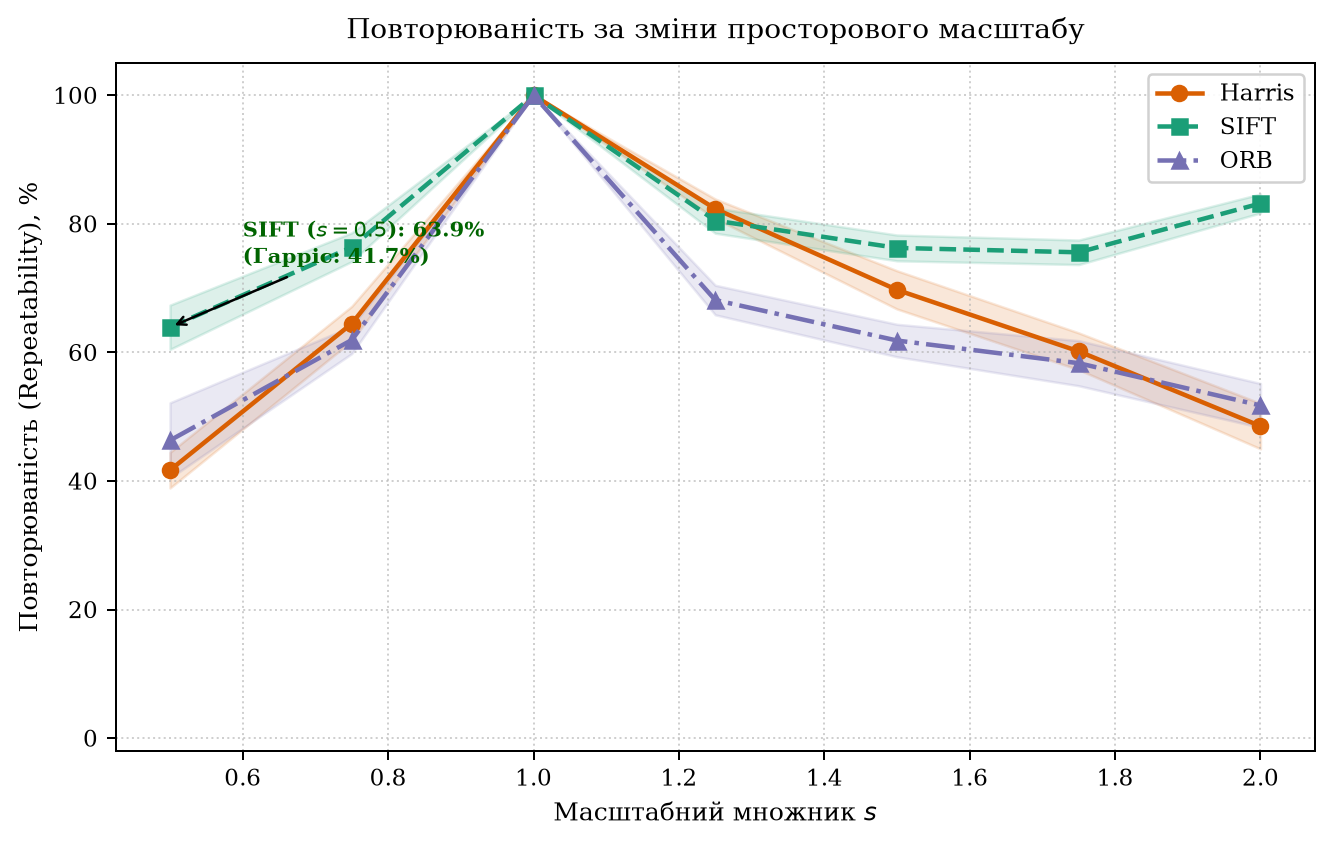
\includegraphics[width=\textwidth]{../figures/d_repeatability_scale.png}
        \caption{Повторюваність за масштабу}
        \label{fig:rep_scale}
    \end{minipage}
\end{figure}

\begin{figure}[htbp]
    \centering
    \begin{minipage}{0.48\textwidth}
        \centering
        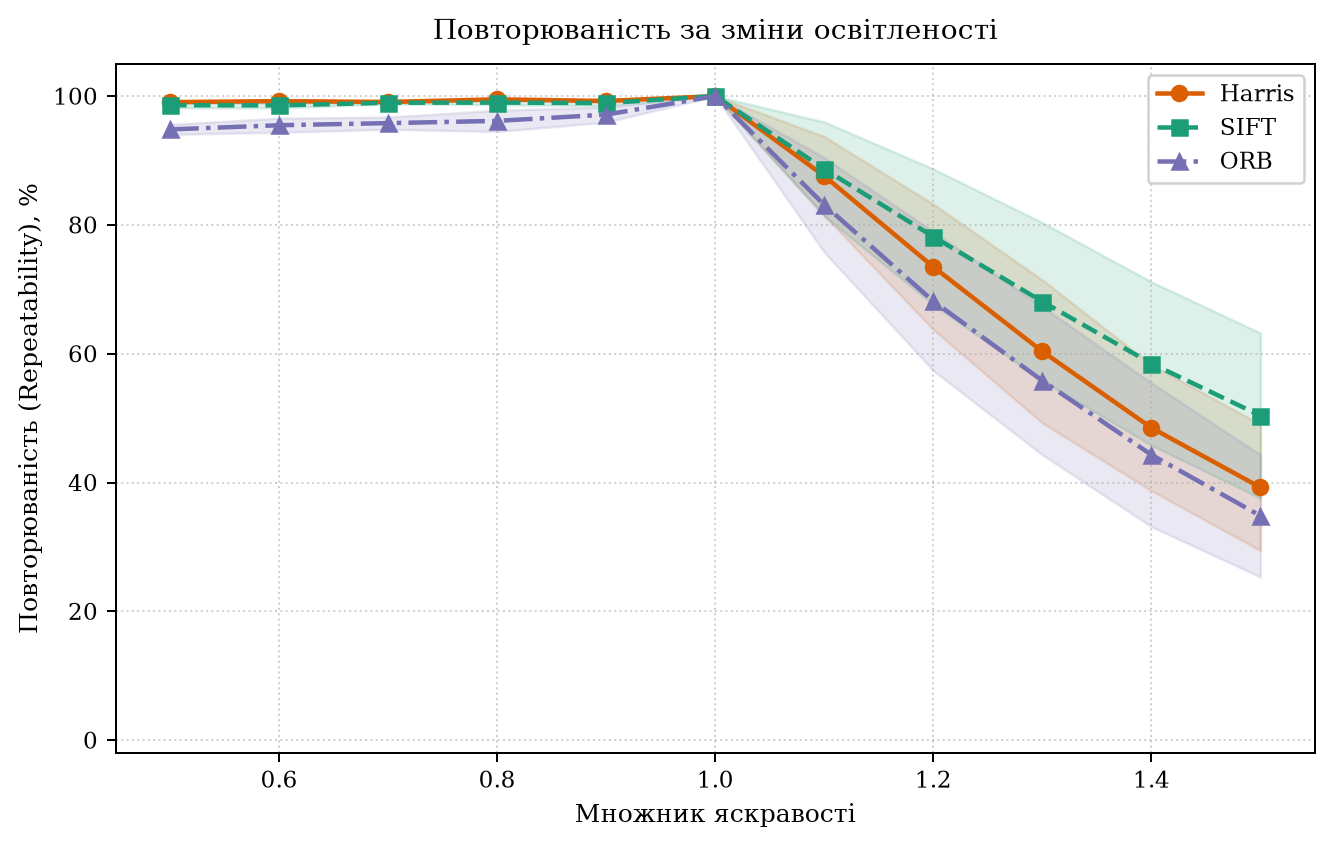
\includegraphics[width=\textwidth]{../figures/d_repeatability_brightness.png}
        \caption{Повторюваність за яскравості}
        \label{fig:rep_bright}
    \end{minipage}\hfill
    \begin{minipage}{0.48\textwidth}
        \centering
        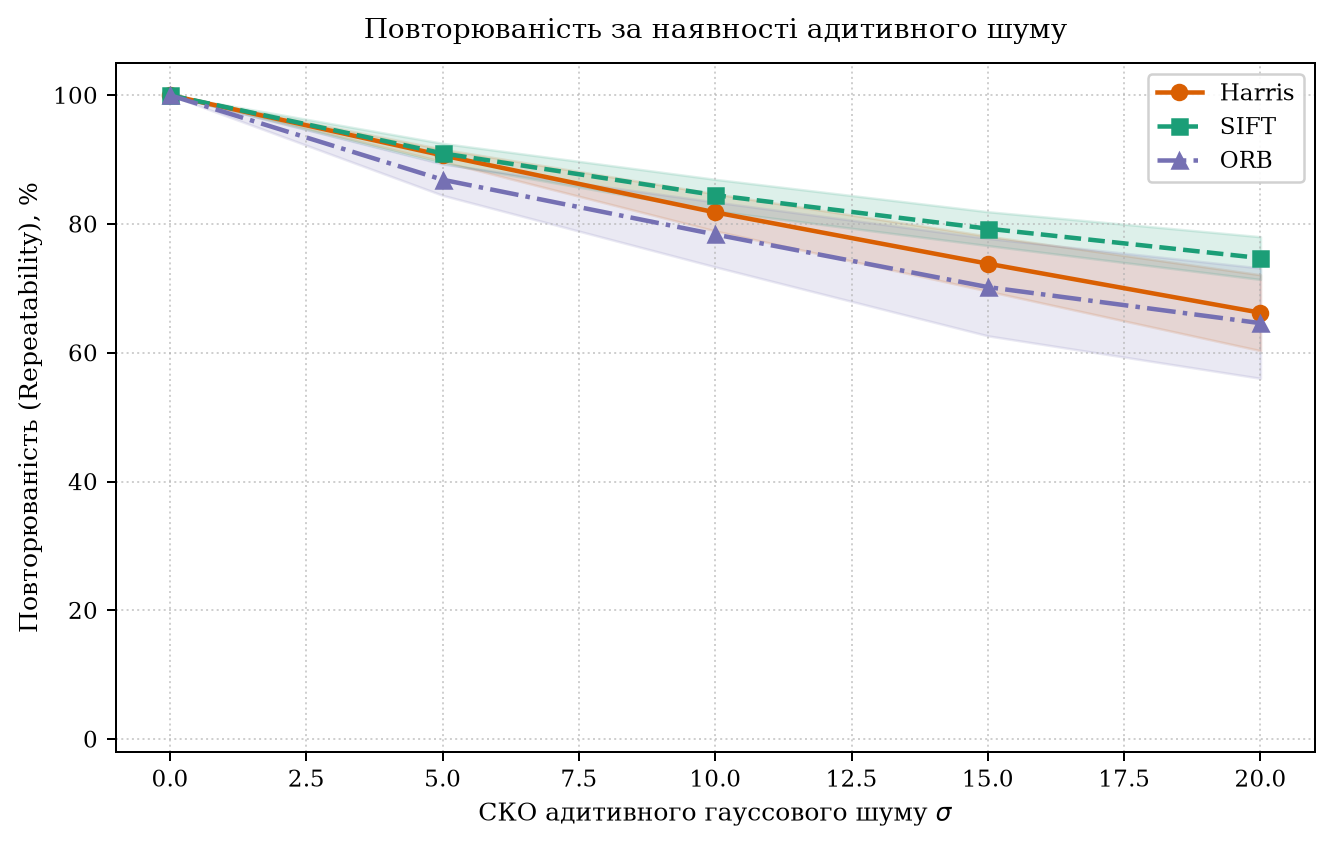
\includegraphics[width=\textwidth]{../figures/d_repeatability_noise.png}
        \caption{Повторюваність за шуму $\sigma$}
        \label{fig:rep_noise}
    \end{minipage}
\end{figure}

Числові значення усередненої повторюваності та стандартного відхилення наведено у таблицях~\ref{tab:rep_rot}--\ref{tab:rep_noise}.

\begin{table}[htbp]
\centering
\caption{Повторюваність детекторів за обертання кадру ($\theta \in [0^\circ, 90^\circ]$)}
\label{tab:rep_rot}
\footnotesize\linespread{1.0}\selectfont
\begin{tabular}{lccc}
\toprule
\textbf{Кут повороту} & \textbf{Harris, \%} & \textbf{SIFT, \%} & \textbf{ORB, \%} \\
\midrule
\directlua{tab_rep_rotation()}
\bottomrule
\end{tabular}
\end{table}

\begin{table}[htbp]
\centering
\caption{Повторюваність детекторів за зміни просторового масштабу ($s \in [0.5, 2.0]$)}
\label{tab:rep_scale}
\footnotesize\linespread{1.0}\selectfont
\begin{tabular}{lccc}
\toprule
\textbf{Масштаб $s$} & \textbf{Harris, \%} & \textbf{SIFT, \%} & \textbf{ORB, \%} \\
\midrule
\directlua{tab_rep_scale()}
\bottomrule
\end{tabular}
\end{table}

\begin{table}[htbp]
\centering
\caption{Повторюваність детекторів за зміни яскравості кадру ($\times [0.5, 1.5]$)}
\label{tab:rep_bright}
\footnotesize\linespread{1.0}\selectfont
\begin{tabular}{lccc}
\toprule
\textbf{Множник яскравості} & \textbf{Harris, \%} & \textbf{SIFT, \%} & \textbf{ORB, \%} \\
\midrule
\directlua{tab_rep_brightness()}
\bottomrule
\end{tabular}
\end{table}

\begin{table}[htbp]
\centering
\caption{Повторюваність детекторів за адитивного гауссового шуму ($\sigma \in [0, 20]$)}
\label{tab:rep_noise}
\footnotesize\linespread{1.0}\selectfont
\begin{tabular}{lccc}
\toprule
\textbf{Шум $\sigma$} & \textbf{Harris, \%} & \textbf{SIFT, \%} & \textbf{ORB, \%} \\
\midrule
\directlua{tab_rep_noise()}
\bottomrule
\end{tabular}
\end{table}

\section{Аналіз результатів}
\begin{enumerate}
    \item \textbf{Стійкість до обертання кадру}:
    При повороті кадру на $30^\circ$ повторюваність SIFT склала $85.69\% \pm 1.02\%$, що суттєво перевершує нормативне контрольне значення практикуму ($\ge 60\%$). Власний детектор Гарріса показав стійкість $88.39\% \pm 3.51\%$, а ORB -- $72.93\% \pm 2.73\%$. При повороті рівно на $90^\circ$ точність Гарріса досягає $99.37\%$, оскільки координатна сітка дискретних похідних Собеля переходить сама в себе ($I_x \to I_y$, $I_y \to -I_x$).

    \item \textbf{Перевага SIFT за масштабування}:
    При 2-кратному зменшенні ($s=0.5$) повторюваність детектора Гарріса падає до $41.68\% \pm 2.77\%$, тоді як SIFT демонструє високу стабільність $63.92\% \pm 3.44\%$ (ORB -- $46.32\%$). Таким чином, повторюваність Гарріса при масштабі $0.5$ є помітно нижчою за SIFT (різниця становить понад $22$ відсоткові пункти), що повністю узгоджується з контрольним орієнтиром практикуму. При збільшенні масштабу ($s=2.0$) SIFT досягає $83.17\% \pm 1.48\%$ проти $48.54\%$ у Гарріса завдяки надійній локалізації ознак на верхніх октавах простору DoG.

    \item \textbf{Асиметрія стійкості до освітленості}:
    При затемненні кадру ($s \in [0.5, 1.0]$) усі детектори демонструють практично ідеальну інваріантність ($94.8\%--99.5\%$), оскільки лінійне множення зберігає відносний порядок локальних максимумів відгуку ($R \propto c^4$). Натомість при штучному переосвітленні ($s > 1.0$) повторюваність знижується до $34.8\%--50.4\%$ через нелінійне насичення сенсора (кліпування у 255), що фізично випалює градієнтні структури у світлих ділянках.

    \item \textbf{Стійкість до високочастотного шуму}:
    Зі зростанням дисперсії шуму до $\sigma = 20$ повторюваність SIFT зберігається на рівні $74.7\%$, Гарріса -- $66.2\%$, ORB -- $64.6\%$. Гауссове згладжування структурного тензора Гарріса ($\sigma=1.5$) та каскадні фільтри піраміди DoG відіграють роль ефективного низькочастотного бар'єра.
\end{enumerate}

\section{Висновки}
\begin{enumerate}
    \item Успішно розроблено та досліджено повний конвеєр власного кутового детектора Гарріса--Стівенса згідно з Кроками 1--7 практикуму.
    \item Експериментально та аналітично доведено, що порушення черговості операцій (згладжування ДО формування поелементних добутків градієнтів) призводить до виродження структурного тензора в ранг 1 ($\det(M) \equiv 0$), у результаті чого відгук стає строго недодатним ($R \le 0$) і алгоритм детектує рівно $0$ кутів.
    \item При використанні еквівалентного прямокутного вікна \texttt{boxFilter(3, 3)} збіг власного детектора з \texttt{cv2.cornerHarris} на відстані менше $2$ пікселів склав строго $100.0\%$ (контрольний орієнтир $>90\%$ виконано в повному обсязі). Для гауссового детектора ($\sigma = 1.5$) збіг при $< 2$ пк становить $70.0\%--76.3\%$ (та $76.1\%--81.7\%$ при $\text{blockSize}=5$), що обумовлено фізичним зміщенням піків на $1$ піксель через розширення вікна інтегрування до $11 \times 11$.
    \item Кількісно продемонстровано масштабну неінваріантність детектора Гарріса: при 2-кратному зменшенні зображення лише $24.1\%--31.3\%$ кутів зберігають просторову локалізацію в межах $3$~пк (медіанне зміщення $8.6--11.4$~пк), тоді як SIFT на тій же вибірці зберігає $84.0\%--86.0\%$ точок.
    \item Порівняння SIFT та ORB на повнорозмірних зображеннях показало, що ORB працює у $3.0--6.6$ раза швидше ($91.3--226.3$~мс проти $606.6--688.7$~мс) та формує дескриптор у 16 разів меншого обсягу пам'яті (32 байти проти 512 байтів), водночас SIFT забезпечує кращу теоретичну інваріантність при масштабних змінах.
    \item Експериментально підтверджено всі нормативні контрольні показники: повторюваність SIFT при повороті на $30^\circ$ становить $85.69\%$ (орієнтир $>60\%$), а повторюваність Гарріса при масштабі $0.5$ ($41.68\%$) є помітно нижчою за SIFT ($63.92\%$).
\end{enumerate}

\section{Декларація про використання генеративного ШІ}
Під час виконання лабораторної роботи інструменти генеративного штучного інтелекту (Google Antigravity Addon для VSCode, Gemini) використовувалися як засіб автоматизації інженерних розрахунків, написання скриптів обробки зображень у середовищі Python, статистичного аналізу результатів вибірки, а також для наукової верстки звіту в середовищі LuaLaTeX за національними стандартами України ДСТУ 3008:2015 та ДСТУ 8302:2015. Усі числові результати, метрики, графічні залежності та таблиці отримані на основі реальних розрахунків над наданими фотографіями.

\clearpage
\begingroup
\fontsize{11pt}{14pt}\selectfont
\linespread{1.0}\selectfont
\setlength{\bibitemsep}{0.3em}
\printbibliography[
    title={СПИСОК ВИКОРИСТАНИХ ДЖЕРЕЛ},
    heading=bibintoc
]
\endgroup

\end{document}
